\documentclass[draft,ms]{agujournal2019}

\usepackage{url} %this package should fix any errors with URLs in refs.
\usepackage{amsmath}
\usepackage{graphicx}
\usepackage{epstopdf}
% \epstopdfDeclareGraphicsRule{.pdf}{png}{.png}{convert -density 40 #1 \OutputFile}
% \DeclareGraphicsExtensions{.png,.pdf}
\usepackage{upgreek}
\usepackage{subcaption}
\usepackage{bm}
\usepackage{float}
\usepackage{multirow}
\usepackage{enumitem}

\usepackage[inline]{trackchanges} %for better track changes. finalnew option will compile document with changes incorporated.
\usepackage{soul}
\linenumbers

\draftfalse


\journalname{Journal of Advances in Modeling Earth Systems (JAMES)}


\begin{document}


\title{Snow equi-temperature metamorphism described by a phase-field model applicable on micro-tomography images: prediction of microstructural and transport properties}
% \textit{Application of a phase-field model on micro-scale snow equi-temperature metamorphism: prediction of microstructural and physical properties}


\authors{L. Bouvet\affil{1,2}, N. Calonne\affil{1}, F. Flin\affil{1}, and C. Geindreau\affil{2}}

\affiliation{1}{Univ. Grenoble Alpes, Université de Toulouse, Météo-France, CNRS, CNRM, Centre d’Études de la Neige, 38000 Grenoble, France}
\affiliation{2}{Univ. Grenoble Alpes, CNRS, Grenoble INP, 3SR, Grenoble, France}

\correspondingauthor{Lisa Bouvet}{lisa.bouvet@univ-grenoble-alpes.fr}

\begin{keypoints}
\item A phase-field model of mean curvature flow is applied on the process of sublimation-deposition describing equi-temperature metamorphism.
\item The model is calibrated through the condensation coefficient parameter by fitting experimental and simulated data at -2$^\circ$C.
\item Equi-temperature metamorphism is predicted on different snow microstructures; morphological and transport properties changes are analyzed.
\end{keypoints}


\begin{abstract}

Representing snow equi-temperature metamorphism (ETM) is key to model the evolution and properties of the snow cover. Recently, a phase-field model describing mean curvature flow evolution on 3-D microstructures was proposed \cite{bretin_phase-field_2019}. In the present work, this model is used to simulate ETM at the pore scale, considering the only process of moving interfaces by sublimation-deposition driven by curvatures. We take 3-D micro-tomographic images of snow as input in the model and obtain a time series of simulated microstructures as output. Relating the numerical time, as defined in the model, to the real physical time involves the condensation coefficient, a poorly-constrained parameter in literature. A calibration was performed by fitting simulations to experimental data through the evolution of specific surface area (SSA) of snow under ETM at -2°C. A condensation coefficient value of $(9.8\pm0.7)10^{-4}$ is obtained and used in all the following simulations. We show that the calibrated model enables to well reproduce an independent time series of ETM at -2°C in terms of SSA, covariance length, and mean curvature distribution. Finally, the calibrated model is used to investigate the effect of ETM on microstructure and effective transport properties (thermal conductivity, vapor diffusion, permeability), for four different snow types. As an interesting preliminary result, simulations show an enhancement of the structural anisotropy of snow in the case of initially anisotropic microstructures such as depth hoar. Results highlight the potential of such micro-scale models for the development of snow property predictions for large-scale snowpack models.


\end{abstract}

\section*{Plain Language Summary}

Snow on the ground is a skeleton of ice and air evolving continuously under different environmental constraints. Among them, equi-temperature metamorphism (ETM) refers to the smoothing and rounding of the snow structure. It is one of the main mechanisms of snow evolution and its correct representation is crucial. Here, we use a mean curvature flow model, describing the smoothing of 3-D microstructures, to simulate ETM of snow. 3-D micro-tomographic images of snow samples are used as input; the output is a time series of 3-D images showing ETM evolution. Describing ETM classically relies on the condensation coefficient, a poorly constrained parameter, that drives the intensity of the evolution. We estimate this parameter for ETM at -2°C by fitting simulations to experimental data. Based on comparisons with an independent dataset, we show that the model enables to well reproduce ETM at -2°C when no significant densification occurs. Finally, we use the model to investigate the effect of ETM on microstructure and effective transport properties of snow for four different snow types. Overall, this work presents promising tools for snow metamorphism study and the development of predictive means for large-scale snow models.

\section{Introduction}
\label{sec:intro}
Dry snow laying on the ground is a complex material made of an ice skeleton in an air matrix that undergoes continuous transformations. Especially, snow evolves through processes of mass redistribution due to thermodynamic mechanisms called snow metamorphism. Different types of snow metamorphism take place depending on the temperature and humidity conditions as well as on the snow microstructure itself. Considering metamorphism is key as it impacts snowpack physical properties, including mechanical properties involved in avalanche processes or thermo-physical properties that drive the surface energy budget of snowpacks \cite{lehning_physical_2002, vionnet_detailed_2012}.\\

Equi-temperature metamorphism (ETM), also referred to as isothermal metamorphism, occurs in snow in quasi-isothermal conditions and is driven by curvature gradients at the ice-air interface. Low curvature ice surfaces have a lower saturation water vapor density than the high curvature ones. Those curvature gradients lead thus to gradients of saturation vapor density causing vapor transfer across the pores (e.g. diffusion) as well as phase changes (sublimation and deposition). Ice sublimates in higher curvature surfaces while water vapor deposits on lower curvature surfaces. 
The overall structure of snow gets rounder, coarser, and more sintered \cite{colbeck_thermodynamics_1980}. These morphological changes come together with mechanical grain rearrangement leading to snow settling. The resulting type of snow is referred to as rounded grains (RG) by \textit{The International Classification for Seasonal Snow on the Ground} \cite{fierz2009international}. Equi-temperature metamorphism is constantly taking place in snow but at different levels of intensity. The higher the contrast in curvature and the higher the snow temperature, the more active the equi-temperature metamorphism. In the presence of high temperature gradients, the influence of curvature effects becomes insignificant as the effect of the temperature gradient metamorphism (TGM) predominates.\\

Modeling the physical processes of metamorphism at fine scale requires the description of the snow microstructure and its evolution (moving interfaces) as well as water vapor transport across the microstructure. Models can be applied on simplified geometry, as in the work of \citeA{miller_microstructural_2003} who considered a 2D regular network of spherical grains. They can also take as input real snow microstructures, for example 3-D images of elementary representative volume (REV) of snow obtained from micro-tomography ($\upmu$CT). To enable micro-scale 3-D modeling, different hypotheses can be used, describing kinetics at the interface, with or without vapor diffusion and settling. \citeA{flin_full_2003} considered fully curvature-driven ETM based on the kinetic limited assumption, and simulated it with an iterative method on 3-D tomographic images. Comparisons between modeled and experimental microstructures were also shown. Also, a first simple grain rearrangement model was used to account for settling \cite{flin2004snow}. Similarly, \citeA{vetter_simulating_2010} used a Monte-Carlo algorithm to simulate the isothermal metamorphism with the kinetic limited assumption and implemented a simple settling model. They obtained consistent results with observations although the model rely on experimental fitting.\\
Recently, phase-field models have been developed to handle the numerical cost and complexity of 3-D micro-scale models \cite{bretin_phase-field_2019,granger_physique_2019, kaempfer_phase-field_2009}. \citeA{kaempfer_phase-field_2009} suggested a phase-field model for snow metamorphism considering interface kinetics and diffusion. They were pioneers with the phase-field method applied to snow metamorphism, and their results are consistent with observations. However, evaluations are qualitative and limited only to one temperature gradient case, mainly because of the numerical cost of the model. 
\citeA{bretin_phase-field_2019} developed a very efficient phase-field multi-phase growth model for curvature-driven interface evolution, which is typically relevant for ETM.\\
Modeling the physics of snow growth classically relies on a condensation parameter $\alpha$ \cite<e.g.,>{ flin_full_2003, kaempfer_phase-field_2009, libbrecht2005physics, yokoyama1990pattern}. This parameter embodies the surface physics that governs how water molecules are incorporated into the ice lattice and is thus key to model metamorphism. The $\alpha$ coefficient ranges from 0 to 1. One can think of $\alpha$ as a sticking probability, equal to the probability that a water vapor molecule striking the ice surface becomes assimilated into the crystal lattice \cite{furukawa2015snow, libbrecht2005physics}. However, it is still poorly understood and quantified, notably because of its complex dependencies to temperature, humidity and crystalline orientation. Numerous values can be found in the literature, ranging from 10$^{-3}$ to 10$^{-1}$ \cite<e.g.,>{libbrecht_measurements_2013}. The large uncertainty on this coefficient is one of the main limiting factor for metamorphism models accuracy.\\
%
To evaluate 3-D models, simulated images are usually compared to experimental data through microstructural properties that can be calculated on 3-D microstructures. Specific surface area (SSA), growth speed, ice thickness and mean curvature were used in previous studies \cite{flin_full_2003, kaempfer_phase-field_2009, vetter_simulating_2010}. To characterize the anisotropy of the microstructure, an anisotropy ratio was suggested based on the ratio of the horizontal and vertical covariance lengths \cite{lowe2013general}. Distributions of the mean curvature can be computed for the upward facing and downward facing ice surfaces, which can be interesting to identify faceted crystals and depth hoar \cite{calonne_study_2014}.\\

Micro-scale models can be useful to design larger scale models, notably to obtain regressions to predict macroscopic mechanical and physical properties. Estimating those properties is often based on numerical computations of experimental tomographic snow images \cite<e.g.,>{calonne_numerical_2011, calonne_study_2014, courville2010lattice, kaempfer2005microstructural, srivastava2010observation}. However, obtaining experimental images covering the wide range of scenarios of snow evolution encountered in nature is a challenge as it is time consuming. 3-D micro-scale models of snow metamorphism could be an efficient method as those properties can be estimated on simulated images.\\

In this article we intend to go further in the micro-scale modeling of ETM by presenting an efficient phase-field algorithm applicable on tomographic images of snow and by calibrating it through the condensation coefficient parameter at -2°C. Using the model, we investigated the evolution of both microstructural and macro-scale transport properties computed on simulated images. Good agreements are reported when compared to an independent dataset of ETM at -2°C as well as common estimates of the literature. 
The paper is organized as follows. The physics of ETM and the phase-field description of the model are described in Section \ref{sec:method}. An overview of the tools used for snow analysis and for the model calibration are also presented in this section. Evaluation of the calibrated model and ETM prediction for different snow microstructures are investigated in section \ref{sec:results}. Section \ref{sec:disc} discusses the model artefacts and the different results of the paper. Finally, Section \ref{sec:conclusion} concludes the manuscript. 

\section{Method}
\label{sec:method}
\subsection{Model}
\label{subsec:model}


\begin{figure}
    \centering
    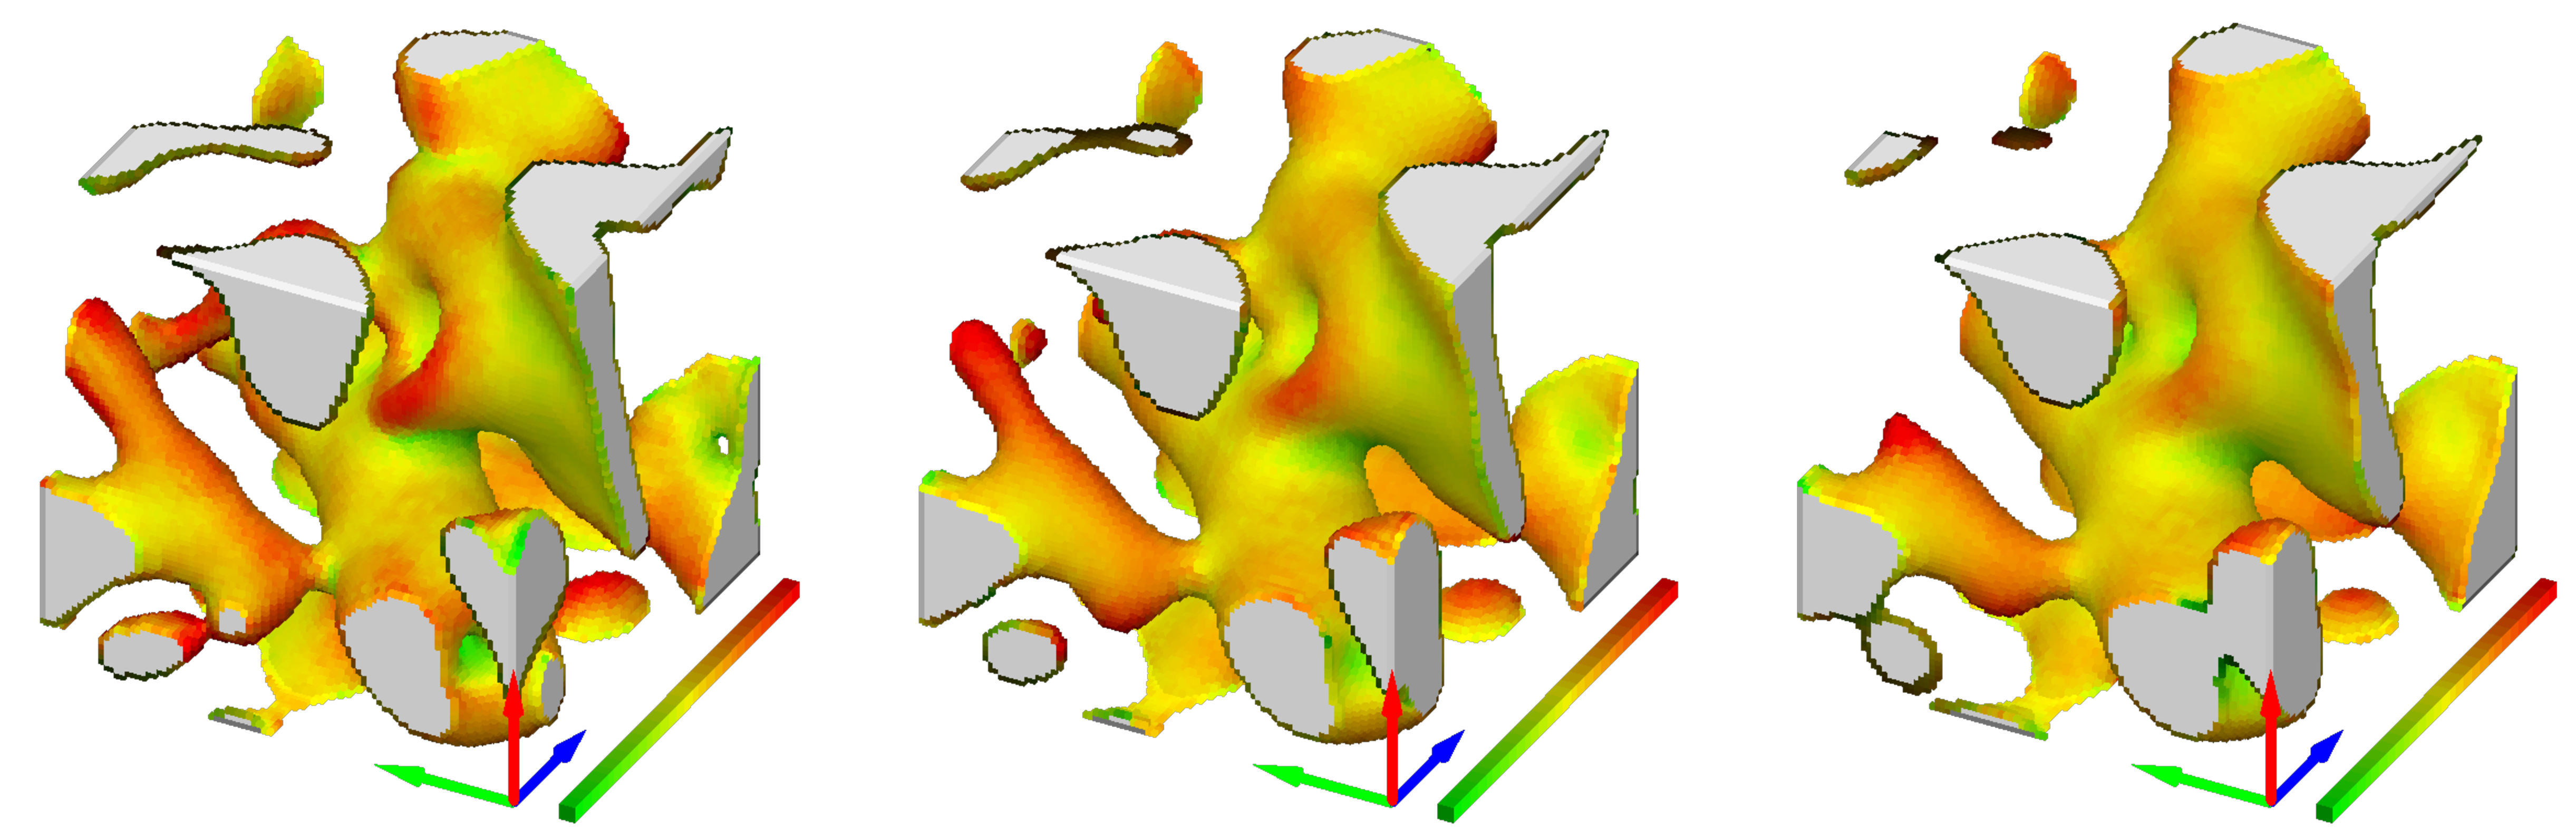
\includegraphics[width=\linewidth]{Figures/eboni_sous_volumes_simu.pdf}
    \caption{3D representation of a tomographic snow sample from \protect\citeA{hagenmuller_motion_2019} under the ETM model Snow-3D after 0, 8 and 16 days at -2$^\circ$C. Concave surfaces are shown in green, convex surfaces in red and flat surfaces in yellow.}
    \label{fig:eboni_sous_volume}
\end{figure}

%PHASE FIELD ET MODELE NUMERIQUE
The phase-field model of \citeA{bretin_phase-field_2019} simulates a multi-phase medium evolving under mean curvature flow and volume conservation of each phase. This flow is defined by an interface evolution where the normal velocity $v_n$ is proportional to the local interface curvature $C$. In our case, we consider two phases where the model minimizes local curvatures while conserving the average of the sample mean curvature (equivalent to mass conservation of the ice phase). The morphological transformations induced by the mean curvature flow can be interpreted as ``smoothing" surfaces and is typically well-suited to model ETM as it is based on the same mathematical description. 

% APPLICATION A LA NEIGE (EQUATIONS ETC)
We apply the model of \citeA{bretin_phase-field_2019} to ETM. This implies that we assume the kinetic-limited metamorphism: vapor transport in the pore space (diffusion) is not described. The latter is considered instantaneous, so that vapor density in air is constant and at equilibrium with temperature and with the ambient sample mean curvature. Also, temperature is considered isotropic and constant. Finally, the model does not include any mechanics and the settling of the ice grains is thus not represented here.\\

Under those conditions, ETM is classically described by the set of equations that follows \cite<e.g.>{flin_full_2003, kaempfer_phase-field_2009}. All the variables, together with the used values and units, are presented in Table \ref{tab:variables}.\\
\begin{subequations}\label{eq:hertz_knu}
\begin{align}
v_{n} &= \alpha v_{\mathrm{kin}} \frac{\rho_{vs}^{\mathrm{amb}} - \rho_{v s}^{\Gamma}}{\rho_{v s}^{ \Gamma }}\quad \text{on}\ \Gamma
\end{align}
\begin{align}
\text{with } v_{\mathrm{kin}} &= \frac{\rho_{v s}^{\mathrm{ref}}}{\rho_i}\sqrt{\frac{k T}{2 \pi m}} % vérifier la formulation de vkin ?
\end{align}
\end{subequations}
%
\begin{subequations}
\begin{align}
\label{equ:gibbsa}
    \rho_{vs}^{\mathrm{amb}}=\rho_{vs}^{\mathrm{ref}}\ e^{d_0 C^{\mathrm{amb}}}
\end{align}
\begin{align}
\label{equ:gibbsb}
    \rho_{vs}^{\Gamma}=\rho_{vs}^{\mathrm{ref}}\ e^{d_0 C} \quad \text{on}\ \Gamma 
\end{align}
\end{subequations}

\noindent Equation \eqref{eq:hertz_knu} is the Hertz-Knudsen equation that describes the normal growth velocity $v_n$ at the interface, such as positive values indicate ice growth and, inversely, negative values indicate ice sublimation. The growth velocity is driven by the difference between the ambient saturation vapor density in the pores $\rho_{vs}^{\mathrm{amb}}$ and the saturation vapor density at the interface $\rho_{vs}^{\Gamma}$. We see in this equation that the interface growth velocity, so the ETM rate, depends linearly on the condensation coefficient $\alpha$.\\

\noindent Equation \eqref{equ:gibbsa} and \eqref{equ:gibbsb} correspond to the Gibbs-Thomson relationship and describe the dependency of saturation vapor density with curvature at a given temperature and using the capillary length $d_0 = \lambda a^3/(k T)$ (m) \cite{kaempfer_phase-field_2009}. Here, Equation \eqref{equ:gibbsa} is used to describe the ambient saturation vapor density in the pores $\rho_{vs}^{\mathrm{amb}}$ in equilibrium with the "ambient" curvature $C^{\mathrm{amb}}$ defined as the average mean curvature of the entire snow volume. Equation \eqref{equ:gibbsb} expresses the interface saturation vapor density $\rho_{vs}^{\Gamma}$ in equilibrium with the local curvature at the interface $C$. Both equations require a reference value of saturation vapor density $\rho_{vs}^\mathrm{ref}$ in air above a flat ice surface (curvature is zero) and at the given temperature. The latter has been largely studied and can be determined as a function of the temperature using existing parameterizations. Here we use the formulation of \citeA{gofflow}, which is appropriated for our range of temperature. Its expression can be found in \citeA{murphy2005review}.

\begin{table}[ht]
\caption{\textit{Notations and values of the physical parameters (above) and variables used in the model (below).}}
\centering
\begin{tabular}{|c|c|c|c|}
\hline \multicolumn{1}{|c} {Symbol} & \multicolumn{1}{|c} { Description } & \multicolumn{1}{|c} { Value, unit } &  \multicolumn{1}{|c|} {Reference} \\
\hline$a$ & mean intermolecular spacing in ice & $3.19 \times 10^{-10}\ \mathrm{m}$ & \citeA{petrenko1999physics}\\
$k$ & Boltzmann's constant & $1.38 \times 10^{-23}\ \mathrm{J\ K}^{-1}$ & \\
$m$ & mass of a water molecule & $2.99 \times 10^{-26}\ \mathrm{kg}$ & \citeA{petrenko1999physics}\\
$\lambda$ & interfacial free energy of ice & $1.09 \times 10^{-1}\ \mathrm{J}\ \mathrm{m}^{-2}$ & \citeA{libbrecht2005physics}\\
$\rho_i$ & density of ice & $917\ \mathrm{kg}\ \mathrm{m}^{-3}$& \\
\hline
T & ETM temperature & -2$^\circ$C &\\
$\alpha$ & condensation coefficient & $(9.8\pm0.7)10^{-4}$ & \\
$n$ & number of model time steps & 4 to 11 &\\
$t_{\mathrm{step}}$ & model time step & 0.5 to 8 & \\
$\varepsilon$ & interface sharpness parameter & $3$ voxels & \citeA{bretin_and_denis_discrete-continuous_2015}\\
\hline
\end{tabular}
\label{tab:variables}
\end{table}


The mean curvature flow model of \citeA{bretin_phase-field_2019} is solved with the phase-field method, which enables an implicit description of the interface using a function that varies smoothly between different phases. When adapted and applied to ETM with two-phases, air and ice, the phase-field equation can be expressed as:\\
\begin{equation}\label{eq:phase-field}\frac{\partial u}{\partial t}(x, t)= d_0 \alpha v_{\mathrm{kin}} \left(\Delta u(x, t)-\frac{1}{\varepsilon^{2}} W^{\prime}(u)\right)\end{equation}
\noindent with $x$ the position, $t$ the time and $u$ the phase function defined as: \begin{equation}\label{eq:phase-func}
u(x,t) := \frac{1}{2}\left(1-\tanh\left(\frac{s}{2}\right)\right)\frac{d(x,t)}{\varepsilon}
\end{equation}
with $s$ the curvilinear abscissa of the phase function, $d$ the distance function from the interface $\Gamma$, $\varepsilon$ the interface sharpness parameter, and $W$ a double-well potential $W(s):= s^{2}(1-s)^{2}/2$. The distance function is linked to the surface local curvature $C$ by $\Delta d(x) = C$ and to the interface normal speed $v_n$ by $\partial_t d (x,t) = - v_n$. By substituting the physical variables to non-dimensional variables such as: $\Tilde{t} = t \alpha v_{\mathrm{kin}} d_0 / d_x^2 $, $\Tilde{x} = x/d_x$ and $\Tilde{\varepsilon} = \varepsilon/d_x$ with $d_x$ (m) the input image resolution, the canonical dimensionless form of equation \eqref{eq:phase-field} is the famous Allen-Cahn equation \cite{bretin_and_denis_discrete-continuous_2015, kaempfer_phase-field_2009}:
% \begin{equation}\label{eq:allen-cahn}\frac{\partial u}{\partial t}(x, t)=\Delta u(x, t)-\frac{1}{\varepsilon^{2}} W^{\prime}(u)\end{equation}
\begin{equation}\label{eq:allen-cahn}\frac{\partial \Tilde{u}}{\partial \Tilde{t}}(\Tilde{x}, \Tilde{t})=\Delta \Tilde{u}(\Tilde{x}, \Tilde{t})-\frac{1}{\Tilde{\varepsilon}^{2}} W^{\prime}(\Tilde{u})\end{equation}
%
% \begin{figure}
%     \centering
%     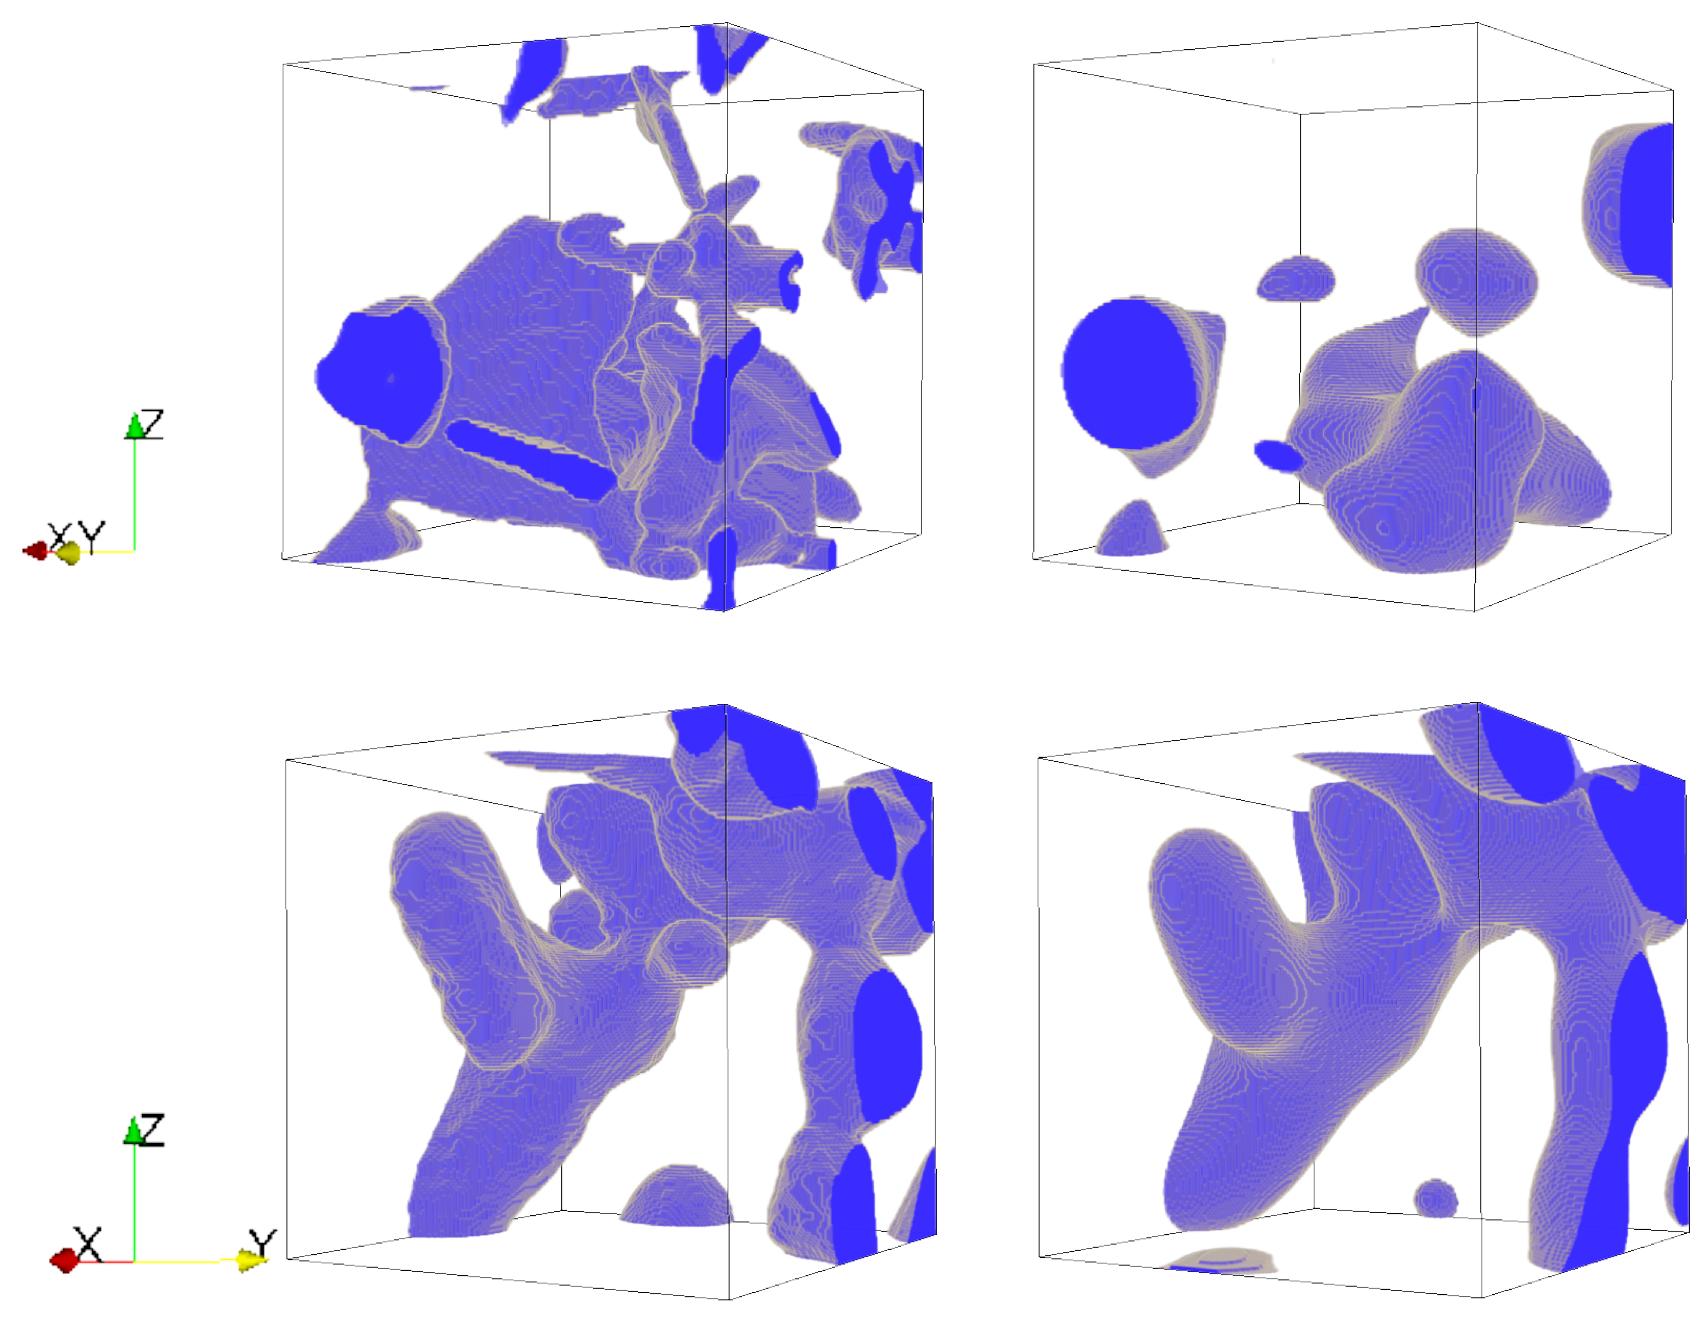
\includegraphics[width=0.7\linewidth]{Figures/disconnections_iso01_iso15.pdf}
%     \caption{Influence of the starting snow type on the disconnections. a) Fresh snow from \protect\cite{flin_three-dimensional_2004} series: initial state (left) and after 40 days of simulation (right) ; b) Sample that underwent 30 days of equi-temperature conditions: initial state (left) and after 40 days of simulation (right) }
%     \label{fig:disco}
% \end{figure}
%
Equation \eqref{eq:allen-cahn} is the general form of the phase-field equation. Note that, in the model, a term is added in the form of a Lagrangian multiplier to guarantee the volume conservation (details can be found in \cite<See>{bretin_phase-field_2019}).


The resulting phase-field model, called Snow-3D, is illustrated in Figure \ref{fig:eboni_sous_volume} with a 16-days simulation of ETM. The model takes as input a 3-D binary image of snow microstructure, such as obtained from tomography, and provides as output a series of 3-D binary images at different time steps of the simulation. In Figure \ref{fig:eboni_sous_volume}, the overall smoothing effect of the curvature-driven evolution can be observed; ice tends to sublimate on the high curvature surfaces (red areas) whereas water vapor deposits on low curvature surfaces (green areas).
The adjustable parameters of the model are the time step $t_{\mathrm{step}}$, the number of time steps $n$ and the interface sharpness parameter $\varepsilon$. Values taken for those parameters are given in Table \ref{tab:variables}. 

% ARTEFACTS
Finally, corrections were necessary to limit some artefacts of the model. First, curvature estimates at the image boundaries can be erroneous, despite the periodic boundary conditions applied on the images. To avoid uncertainties regarding that issue, the edges of the simulated images were cut off by a certain width (0.6 mm) prior to further analysis. Also, as the model does not account for gravity, simulations can lead to create ``floating" ice grains \cite<see>{flin_full_2003, vetter_simulating_2010}, especially for snow in early stages of metamorphism that undergo significant settling \cite{schleef2014influence}. 
% An example of grain disconnections is shown in Figure \ref{fig:disco}. 
To prevent this non-physical phenomenon, we restrict input images to adequate snow microstructures and suppress disconnected ice grains.


\subsection{Calibration} 
\label{subsec:calib}

\begin{table}
\caption{\textit{Above: Experimental time-series of snow images used to calibrate and evaluate the Snow-3D model (Sec. \ref{Section:Calibration}). Density values correspond to the value at the initial stage of the series (0 day). Snow types are the main type reported throughout the time-series, or, when separated by an arrow, are the initial and final type. Below: Experimental snow images taken as input to simulate ETM and predict snow properties (Sec. \ref{sec:prediction}).}}
\begin{tabular}{|c|c|c|c|c|c|}
\hline Name & Metamorphism stage & Resolution & Dimension & Density & Snow types \\
 &  & ($\upmu$m) &(voxel) & (kg m$^{-3}$) &  \\
\hline 
Iso$^\mathrm{a}$ & $84\ \mathrm{days}$ of ETM at $-2^{\circ} \mathrm{C}$ (10 images) & 4.9 & 512 & 158 & \small{$\mathrm{PP} \rightarrow \mathrm{RG}$}\\
Eboni$^\mathrm{b}$ & 4 days of ETM at $-2^{\circ} \mathrm{C}$ (20 images) & 7.5 & 450 & 212 & \small{$\mathrm{DF/RG}$}\\
\hline\hline 
I17$^\mathrm{c}$ & Recent fallen snow & 7.3 & 700 & 147 & \small{$\mathrm{DF}$} \\
TG2$^\mathrm{c}$ & after 16 days at 19 K m$^{-1}$ & 7 & 700 & 254 & \small{$\mathrm{FC} / \mathrm{DH}$} \\
Grad3$^\mathrm{d}$ & after 8 days at 100 $\mathrm{K}\ \mathrm{m}^{-1}$ & 10 & 600 & 372 & \small{$\mathrm{DH}$} \\
7G9m$^\mathrm{e}$ & after 21 days at 43 $\mathrm{K}\ \mathrm{m}^{-1}$ & 9.7 & 950 & 314 & \small{$\mathrm{DH}$} \\
\hline
\end{tabular}
\label{tab:series}
$^\mathrm{a}$\protect\citeA{flin_three-dimensional_2004}. $^\mathrm{b}$\protect\citeA{hagenmuller_motion_2019}.
$^\mathrm{c}$\protect\citeA{dumont2021experimental}.  $^\mathrm{d}$\protect\citeA{flin2011computations}. $^\mathrm{e}$\protect\citeA{calonne_study_2014}.
\end{table}


 The model output is a series of $n$ images separated by a time step $t_{\mathrm{step}}$, without any notion of physical duration. To obtain physical simulation evolution, a calibration step is thus needed.
Considering the non-dimensional time used to deduce the dimensionless equation \eqref{eq:allen-cahn}, the model physical time can be expressed as \cite{bretin_and_denis_discrete-continuous_2015}: 
\begin{equation}\label{equ:alpha}
   t = \frac{\Tilde{t}\ d_x^2}{\alpha v_{\mathrm{kin}} d_0}
\end{equation}
with $t$ the physical time (s) and $\Tilde{t} = t_{\mathrm{step}} \times n$ the simulated time (-). The condensation coefficient $\alpha$ is needed to determine the physical time. To derive a value of $\alpha$, we reproduce the ETM experiment of \citeA{flin_three-dimensional_2004} with the model and compare the simulated series of images with the experimental one (series Iso in Table \ref{tab:series}) using the SSA evolution. The SSA parameter was chosen because it is a good scalar descriptor of the microstructure evolution during ETM.
\\
The series of experimental images of \citeA{flin_three-dimensional_2004} is composed of 10 images showing snow at different times of its evolution during ETM at -2$^\circ$C from 0 to 84 days. Each image was obtained by micro-tomography of a snow sample extruded from a snow slab undergoing ETM. The first images of the series (Iso01, Iso03, Iso04) were not considered at all in this paper as they correspond to fresh snow and would have lead to grain disconnection issues (Sec. \ref{subsec:model}). To calibrate, we use the image Iso05 (day 5), Iso08 (day 12), Iso11 (day18) and Iso15 (day 33). The last three images of the series (Iso19, Iso21, and Iso23) were not selected for calibration as they are close in time to the end of the experiment and so data are too few for relevant statistics when estimating $\alpha$. Finally, during the calibration process, the sides of each simulated image were cut off by a stripe of thickness equal to the size of two heterogeneities (0.6 mm) before the SSA calculation to avoid edge artefacts while keeping volumes larger than the REV being typically about 2.5 mm for SSA \cite<e.g.>{flin2011computations}.\\

\begin{figure}
    \centering
    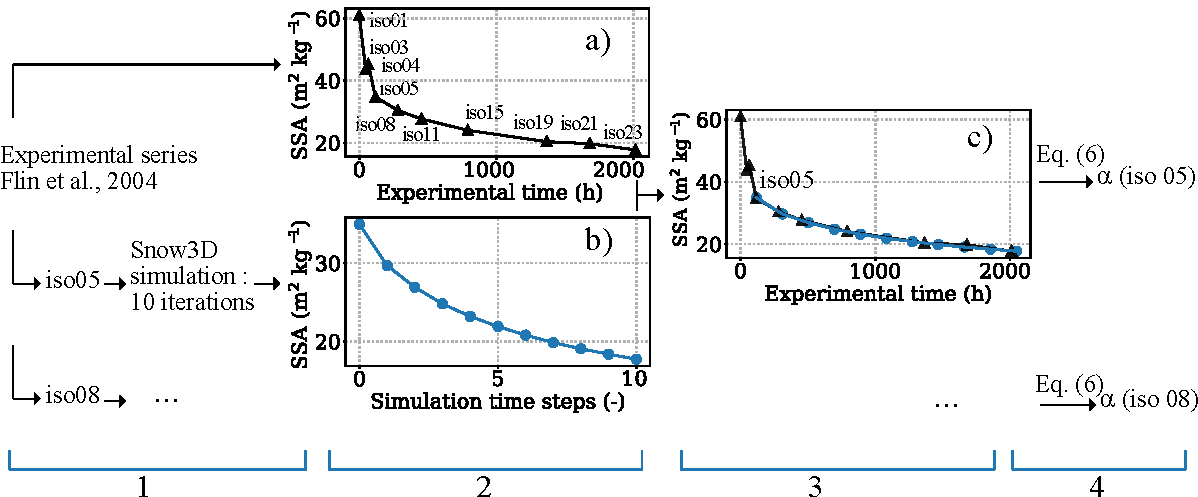
\includegraphics[width = \linewidth]{Figures/workflow_aff_new.pdf}
    \caption{Workflow of the time calibration process and determination of the condensation coefficient.}
    \label{fig:workflow}
\end{figure}

The calibration process is schematized in four steps in Figure \ref{fig:workflow}. For each selected image of the experimental series taken successively as input:
\begin{enumerate}
    \item we run the model with the same parameters ($n$ = 10, $t_{\mathrm{step}}$ = 16, $\varepsilon$ = 3) to obtain a simulated series composed of 10 images. 
    \item we calculate the SSA evolution on the simulated series (Fig. \ref{fig:workflow}.b).
    \item we fit the SSA of the simulated series (Fig. \ref{fig:workflow}.b) to the SSA of the experimental series (Fig. \ref{fig:workflow}.a) by adjusting the time axis. More precisely, we scale the simulation time to the experimental time such that simulated SSA matches best experimental SSA best by minimizing the Root Mean Square Error (RMSE) between the two curves (Fig. \ref{fig:workflow}.c).   
    \item we use the simulated time and the fitted physical time to derive a value of the condensation coefficient $\alpha$ through the equation \eqref{equ:alpha}. 
\end{enumerate}

The average condensation coefficient $\alpha$ and standard deviation were calculated from the four $\alpha$ coefficients obtained from the four images. The resulting condensation coefficient is $\alpha = ( 9.8 \pm 0.7) 10^{-4}$. As the condensation coefficient is strongly temperature dependent and the temperature condition of the experiment of \citeA{flin_three-dimensional_2004} used to calibrate is -2$^\circ$C, the calibrated model can only be used to simulate ETM at this temperature. To evaluate the influence of $\alpha$ on the microstructural parameters, we calculate the variation of the microstructural parameters (SSA, covariance length, and mean curvature) as a function of $\alpha$ variation. In the range of the $\alpha$ derived from the different samples, the parameters only have a maximum alteration of 5\%, which is small compared to the physical precision of those parameters. 

\subsection{Computation of snow properties}
\label{subsec:methode_physical_appli}

To characterize our simulated and experimental microstructures, we calculated on our volumes a range of microstructural and physical properties.

\noindent \textbf{Microstructural properties} 
\begin{itemize}
    \item The snow density $\rho_{\mathrm{s}}$ (kg m$^{-3}$) computed with a simple voxel counting algorithm.
    
    \item The mean curvature (mm$^{-1}$), defined as $\left(C_{min} + C_{max})\right/2$ with $C_{min}$ and $C_{max}$ respectively the minimum and maximum 2-D normal curvatures at one point of the surface. As those values are computed for each point of the surface, they are represented as statistical distributions. Values near 0 mm$^{-1}$ correspond to flat surfaces, positive values to convex surfaces, and negative values to concave surfaces; the higher the values, the more concave or convex the surfaces \cite{ogawa2006representation}. The mean curvature is expressed in terms of occurrence ratio, which gives the percentage of the ice surface area that exhibits a mean curvature located in a particular curvature class.
    
    \item The specific surface area SSA (m$^2$ kg$^{-1}$), defined as the total surface area of ice per unit of mass \cite{dumont2021experimental, flin2011computations}.
    
    \item The covariance (or correlation) length $l_{c}$, calculated along the x-, y-and z- direction of the images, corresponds to the characteristic size of the ice heterogeneities in a given snow microstructure \cite{lowe2013general}. 
    
    \item The anisotropy coefficient
    $\mathcal{A}(\star)$, that can be computed for each microstructural and physical property which are computed along 3 dimensions. This coefficient is defined as the ratio between the vertical component over the horizontal ones, such as $\mathcal{A}(\star)=\star_{z} / \star_{x y}$. The property is considered isotropic if it exhibits a coefficient close to 1, otherwise the property is anisotropic. For example, $\mathcal{A}(l_c)$ largely above 1 means that the covariance length is higher in the vertical direction than in the horizontal one, and thus describes a structure that is vertically elongated.
\end{itemize}


\noindent \textbf{Macro-scale transport properties}$\quad$ The 3-D tensors of the intrinsic permeability $\mathbf{K}$ (m$^2$), of the effective thermal conductivity $\mathbf{k}$ (W m$^{-1}$ K$^{-1}$) and of the effective coefficient of vapor diffusion $\mathbf{D}$ (m$^2$ s$^{-1}$) were computed on a set of simulated 3-D images. For each property, a specific boundary value problem, arising from a homogenization technique \cite{auriault2009homogenization, calonne2015macroscopic}, is solved on the images applying periodic boundary conditions on the external boundaries of each volume using the software Geodict \cite{thoemen_3d_2008}. The effective diffusion coefficient was computed with an artificial diffusion coefficient of gas in free air set to $D^{\mathrm{air}} =$ 1 m$^2$ s$^{-1}$. In this study, we present the normalized values of the effective diffusion $\mathbf{D} / D^{\mathrm{air}}$ (dimensionless). $\mathbf{K}$ is normalized by the equivalent sphere radius $r_{\mathrm{es}}=3/(\mathrm{SSA} \times \rho_{\mathrm{i}})$ to introduce a dimensionless tensor: $\mathbf{K}\mathrm{^{*}} = \mathbf{K}/r_{\mathrm{es}}^2$ \cite{calonne_3D_2012}.
As the non-diagonal terms of the tensor $\mathbf{K}$, $\mathbf{k}$ and $\mathbf{D}$ are negligible, we consider only the diagonal terms, i.e. seen as the eigenvalues of the tensors (the image axes $x$, $y$ and $z$ are the principal directions of the microstructure, $z$ being along the direction of gravity). Besides, the tensors are transversely isotropic as the components in $x$ are very similar to the ones in $y$.
In the following, $K$, $k$ and $D$ refer to the average of the diagonal terms of $\mathbf{K}$, $\mathbf{k}$ and $\mathbf{D}$ respectively. $K_z$, $k_z$ and $D_z$ refer to the vertical components and $K_{xy}$, $k_{xy}$ and $D_{xy}$ refer to the mean horizontal components where $K_{xy} = (K_{x} + K_{y}) /2$, $k_{xy} = (k_{x} + k_{y}) /2$ and $D_{xy} = (D_{x} + D_{y}) /2$. Finally, the anisotropy of the properties is characterized based on the anisotropy ratio $\mathcal{A}(K) = K_z / K_{xy}$, $\mathcal{A}(k) = k_z / k_{xy}$ and $\mathcal{A}(D) = D_z / D_{xy}$ \cite<see e.g.>{calonne_study_2014}.


\section{Results}
\label{sec:results}
\subsection{Model evaluation}
\label{Section:Calibration}

\begin{figure}
    \centering
    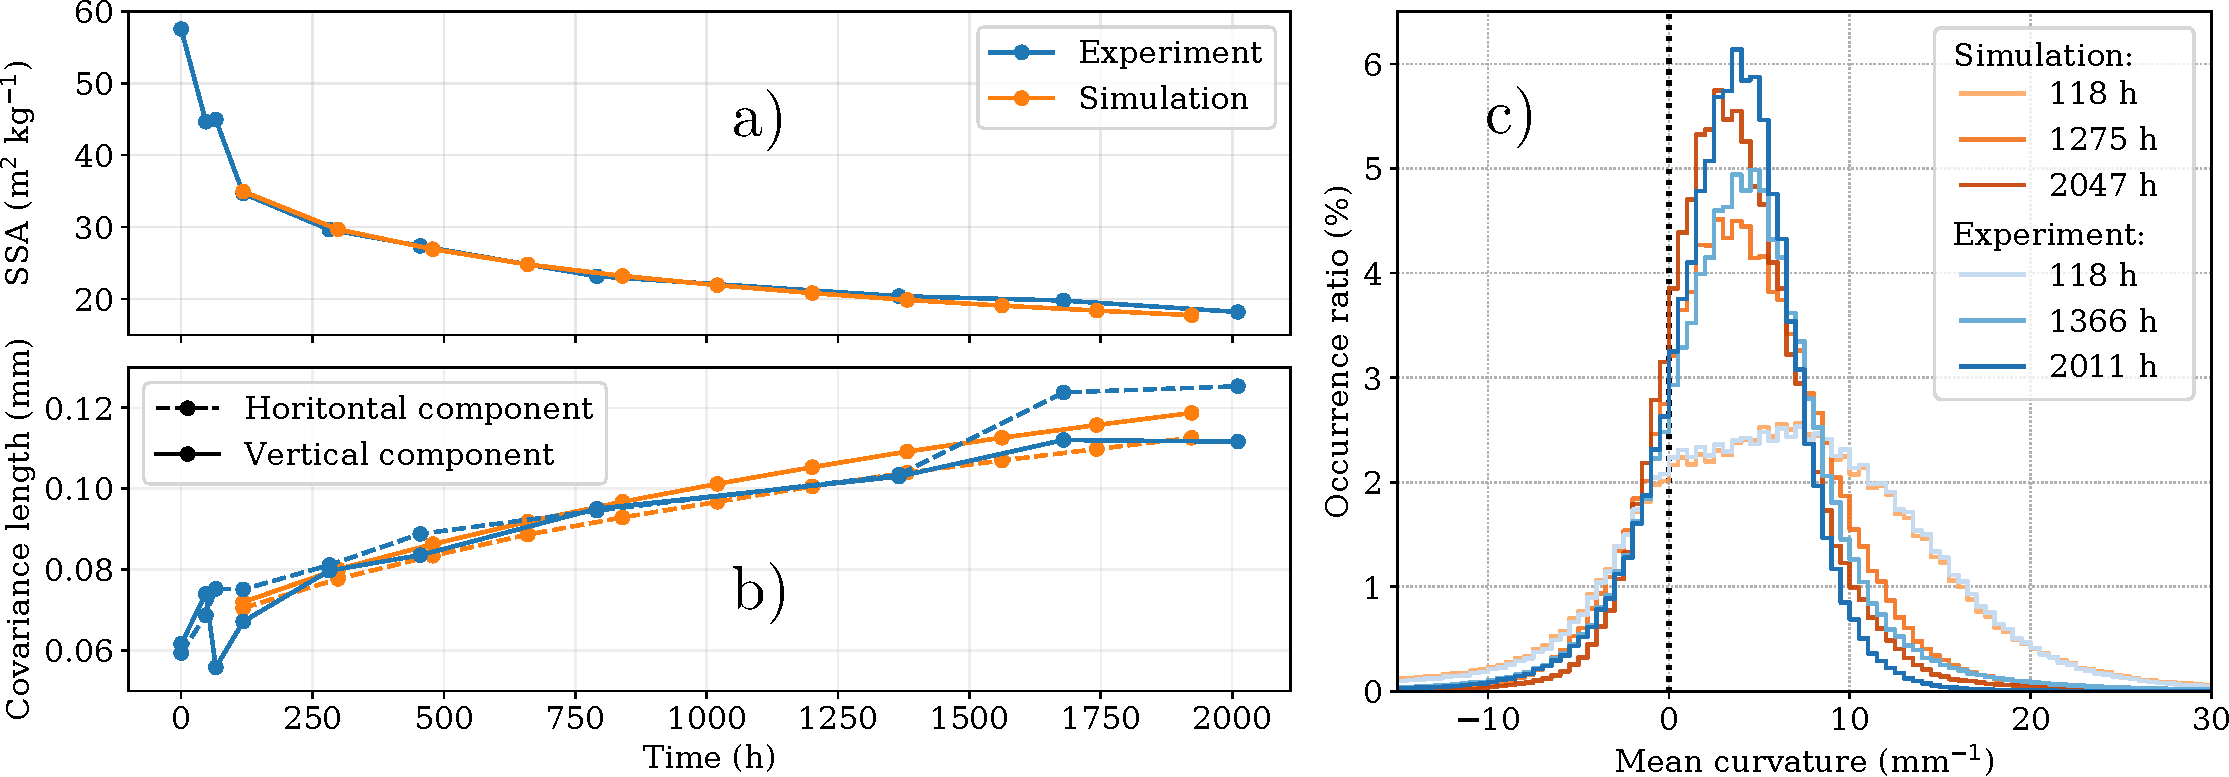
\includegraphics[width=\linewidth]{Figures/microstruct_isoFlin_exp_simu.pdf}
    \caption{Comparison between the experiment of \protect\citeA{flin_three-dimensional_2004} and the simulations, taking the Iso05 sample as the model input. Time evolution of the a) SSA ; b) covariance length ; and c) mean curvature histograms.}
    \label{fig:flin_evaluation}
\end{figure}

Here, we evaluate the calibrated model by comparing experiments and simulations. To do so, we use the experimental series of images of \citeA{flin_three-dimensional_2004}, which was the dataset used to calibrate the model (Sec. \ref{subsec:calib}), as well as the one of \citeA{hagenmuller_motion_2019} to allow for an independent comparison. Evaluations are performed through the SSA, the covariance lengths, and the mean curvature distribution computed from the simulated and experimental images.\\

 The experimental series of images of \citeA{hagenmuller_motion_2019} was obtained as part of a study on dust particles in snow under both temperature gradient and equi-temperature conditions.
 %is a 110 h long experiment of ETM at -2$^\circ$C with 32 tomographic images. The series was used to study dust particles in snow (concentration of 0.5 mg g$^{-1}$) under both temperature gradient and equi-temperature conditions.
 Here we focus on the equi-temperature part of the experiment and select 20 tomographic images from about 70 hours of ETM at -2°C (Eboni in Table \ref{tab:series}). We assume that dust has little influence on ETM (dust concentration of 0.5 mg g$^{-1}$) and artificially convert voxels of dust particles to voxels of air in the images, so we can use them as model inputs. In the work of \citeA{hagenmuller_motion_2019}, the snow sample was observed with in operando X-ray tomography, meaning than the same sample was scanned at regular intervals \cite{calonne2015celldym}. This method enables to compare directly simulated and experimental images, unlike the series of \citeA{flin_three-dimensional_2004} for which each image corresponds to a different snow sample.\\

The evolution of SSA, covariance length and mean curvature from the experiment of \citeA{flin_three-dimensional_2004} and simulated with Snow-3D are shown in Figure \ref{fig:flin_evaluation}. As expected, simulations follow closely the SSA decrease reported in the experiment (Fig \ref{fig:flin_evaluation}.a).
The RMSE is of $0.58\ \mathrm{m}^2\ \mathrm{kg}^{-1}$ for SSA values evolving from 35 to 18 m$^2$ kg$^{-1}$.
Covariance lengths increase over time from around 0.07 to 0.12 mm. This evolution is well reproduced by the model with a small RMSE of $0.005\ \mathrm{mm}$ (Fig. \ref{fig:flin_evaluation}.b). Looking in more details, the snow microstructure gets slightly elongated in the horizontal direction with larger covariance lengths in the horizontal direction than in the vertical one, of about 0.02 mm. This is not captured by the simulations for which differences between vertical and horizontal covariance lengths do not exceed 0.005 mm and remain rather constant over time. 
The mean curvature distribution presented in Figure \ref{fig:flin_evaluation}.c allows to qualitatively compare the evolution of grain surface morphology. We see the distributions are narrowing and shift toward lower mean curvature values, especially in the first time period. This depicts that ice surfaces are getting more uniform toward large rounded grains. Simulations follow closely the experimental data, showing good agreements at each time step. Finally, we should keep in mind that, when evaluating the simulations against the data of \citeA{flin_three-dimensional_2004}, the small disagreements observed might be partly due to the fact that the experimental properties (a) do not only reflect time evolution but also the spatial variability of the monitored snow layer and (b) could be influenced by settling, which is not considered in simulations (Sec. \ref{sec:method}).\\

\begin{figure}
    \centering
    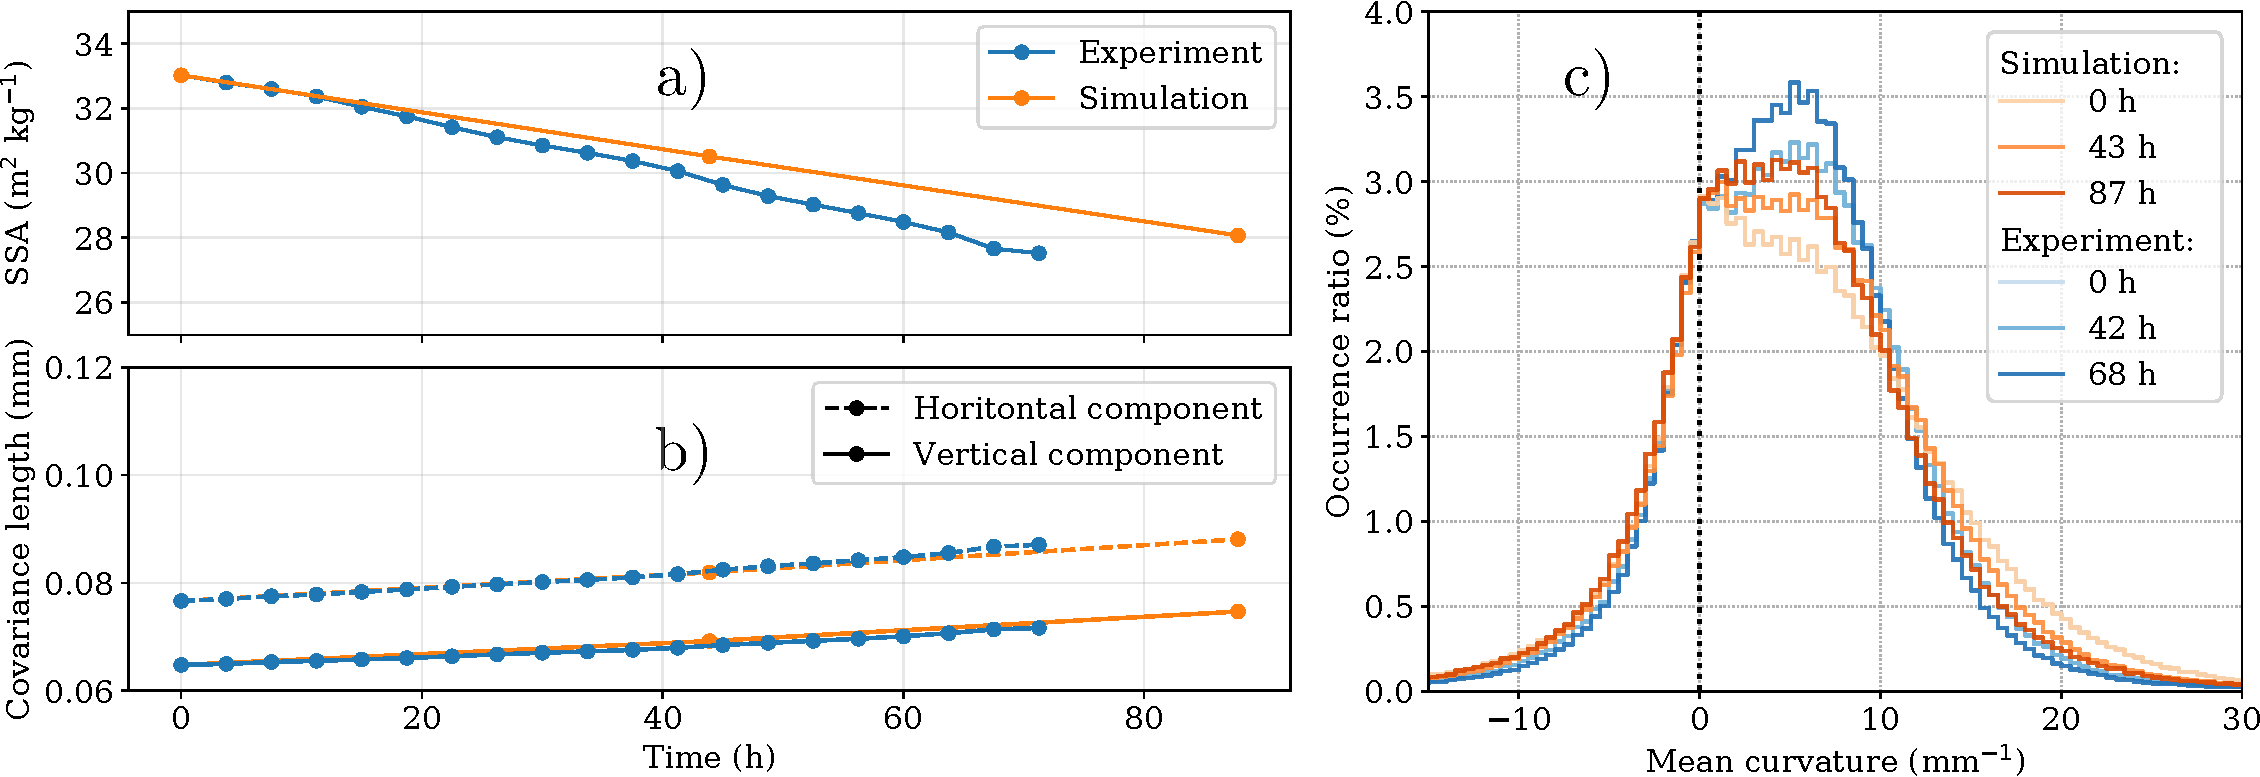
\includegraphics[width=\linewidth]{Figures/microstruct_EBONI_exp_simu.pdf}
    \caption{Comparison between the experiment of \protect\citeA{hagenmuller_motion_2019} and the simulations. Time evolution of the a) SSA ; b) covariance length ; and c) mean curvature histograms.}
    \label{fig:eboni}
\end{figure}

Figure \ref{fig:eboni} shows the model evaluation for the experiment of \citeA{hagenmuller_motion_2019}. As this experiment is rather short compared to the previous one (70 hours), microstructural changes are more subtle. Overall, SSA decreases from 33 to 28 m$^2$ kg$^{-1}$, whereas covariance length increases from 0.077 to 0.087 mm in the horizontal direction and from 0.065 to 0.072 mm in the vertical one. The model performs well for the SSA with a RMSE of $0.79\ \mathrm{m}^2\ \mathrm{kg}^{-1}$ and, even better for the covariance length with a RSME of $0.0003\ \mathrm{mm}$ (mean for both directions).
The rate of SSA decrease seems slightly underestimated by the model, reaching a difference of $1.47\ \mathrm{m}^2\ \mathrm{kg}^{-1}$ after 80 h; this is still small with respect to the SSA value range. Good agreements are in overall found for the mean curvature distribution (Fig. \ref{fig:eboni}.c). \\


\subsection{Model prediction}
\label{sec:prediction}

Here the model is used to predict equi-temperature metamorphism on different snow microstructures (Table \ref{tab:series}). We selected four 3-D experimental images of snow showing various features and used them as input image in the model. The samples are I17 (DF), which present an isotropic structure with rounded shapes, TG2 (FC/DH), Grad3 (DH), and 7G9m (DH). The 3 last images are snow samples that underwent different temperature gradients and show associated features in varying degrees (degree of faceting, degree of structural anisotropy, etc). Simulations were performed with isothermal conditions at -2$^\circ$C and for a condensation coefficient $\alpha$ of $9.8\ 10^{-4}$. It led to 4 series of 4 to 11 images simulating from 70 days to 80 days of ETM. This time range enables to capture the important physical evolution while keeping simulation times close to those of the calibration. Figure \ref{fig:evolutions_3D} illustrates the simulated image series obtained for the 4 samples: a 3D view of the microstructure as well as a vertical slice are shown for each sample at the initial, intermediate, and final stage of the simulation.\\

\begin{figure}
    \centering
    \includegraphics[width =\linewidth]{Figures/evolution_3D_new_textepetit_courr.pdf}
    \caption{Initial, intermediate and final stage of the simulated series of Grad3, 7G9m, TG2 and I17. 3-D views and vertical slices taken at the center of each cube are presented. Concave surfaces are shown in green, convex surfaces in red and flat surfaces in yellow in the 3-D views. The ice phase is colored in yellow and the air phase in grey in the slice representations.}
    \label{fig:evolutions_3D}
\end{figure}

\subsubsection{Microstructural parameters}

\begin{figure}
    \centering
    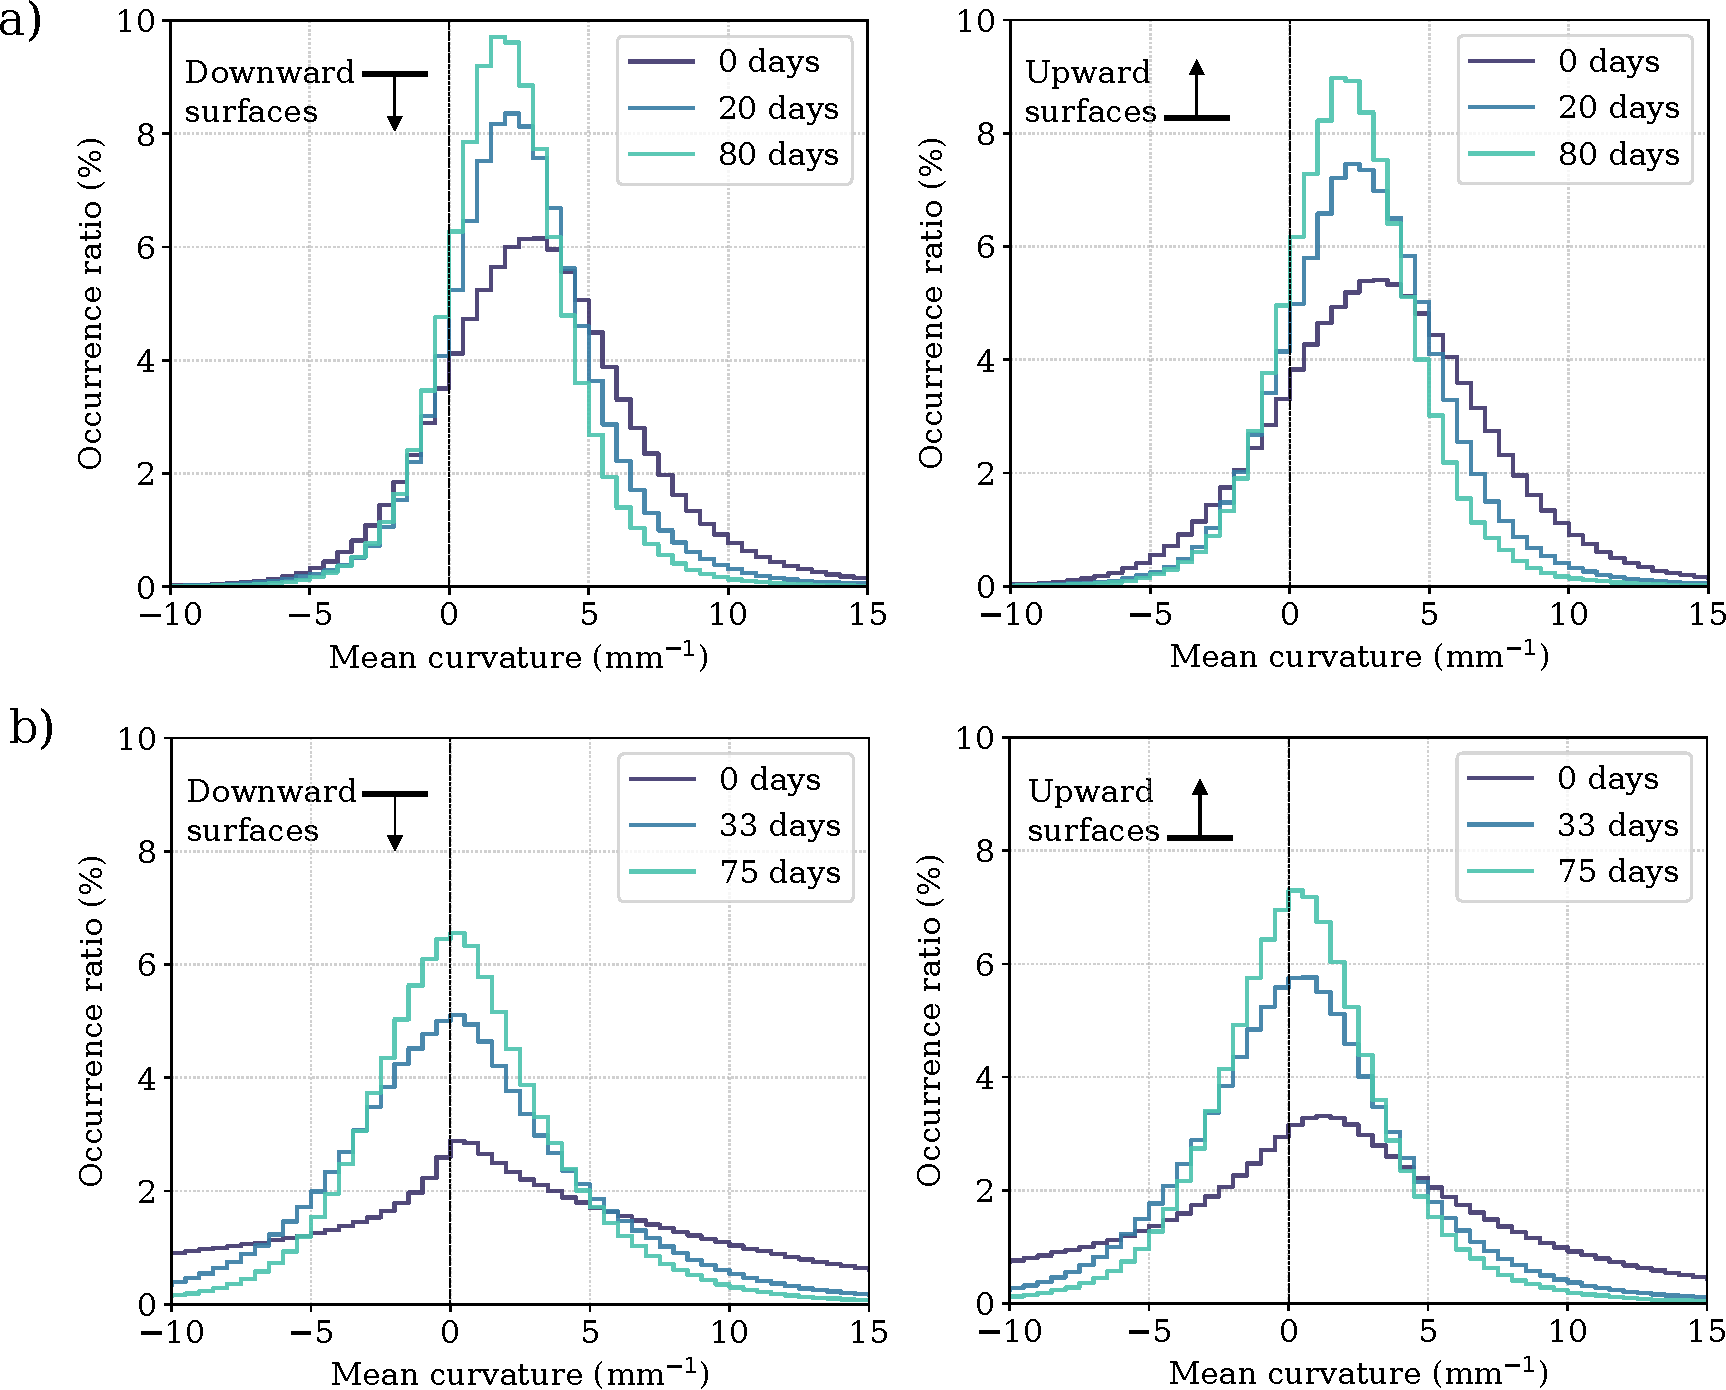
\includegraphics[width=\linewidth]{Figures/histo_i17_grad3_copie_invert.pdf}
    \caption{Time evolution of the mean curvature distribution from the downward (left) and upward (right) surfaces of I17 (a) and Grad3 (b) simulated series. Each curvature class is 0.5 mm$^{-1}$ wide.}
    \label{fig:histo_i17_grad3}
\end{figure}

Figure \ref{fig:histo_i17_grad3} presents the mean curvature distribution evolution for the sample I17 (DF) and Grad3 (DH) (Sec. \ref{subsec:methode_physical_appli}). For I17, the initial upward and downward distributions are similar with a peak of mean curvature located around 4 mm$^{-1}$ and an occurrence ratio of 5 \% (Fig. \ref{fig:histo_i17_grad3}.a). This reflects isotropic rounded ice structures at the initial stage. With time, the area-averaged mean curvature decreases gradually and the distributions are narrower, indicating that the ice structures tend toward larger rounded shapes and become more uniform.\\

For the evolution of Grad3 (Figure \ref{fig:histo_i17_grad3}.b), the initial upward and downward distributions are wider than for the initial stage of I17, revealing a larger variety of shapes. Besides, the initial upward and downward surfaces exhibit clearly distinct distributions: the peak of mean curvature is located around 0 mm$^{-1}$ for the downward ones and at 1.5 mm$^{-1}$ for the upward ones. The near-0 downward distribution depicts the presence of plane surfaces, which are facets as typically found in the lower area of a depth hoar crystal. In contrast, curvatures of the upward-looking surfaces show rather rounded shapes, again as typically observed in the upper area of a depth hoar crystal. With time, the differences between the downward and upward surfaces fade away and both show a narrower distribution (approx. 7 \% occurrence ratio) with a low area-averaged mean curvature. This indicates ice surfaces more uniform that are mostly large and rounded shapes, for both downward and upward surfaces. This overall trend is similar to the one reported for I17.\\

\begin{figure}
    \centering
    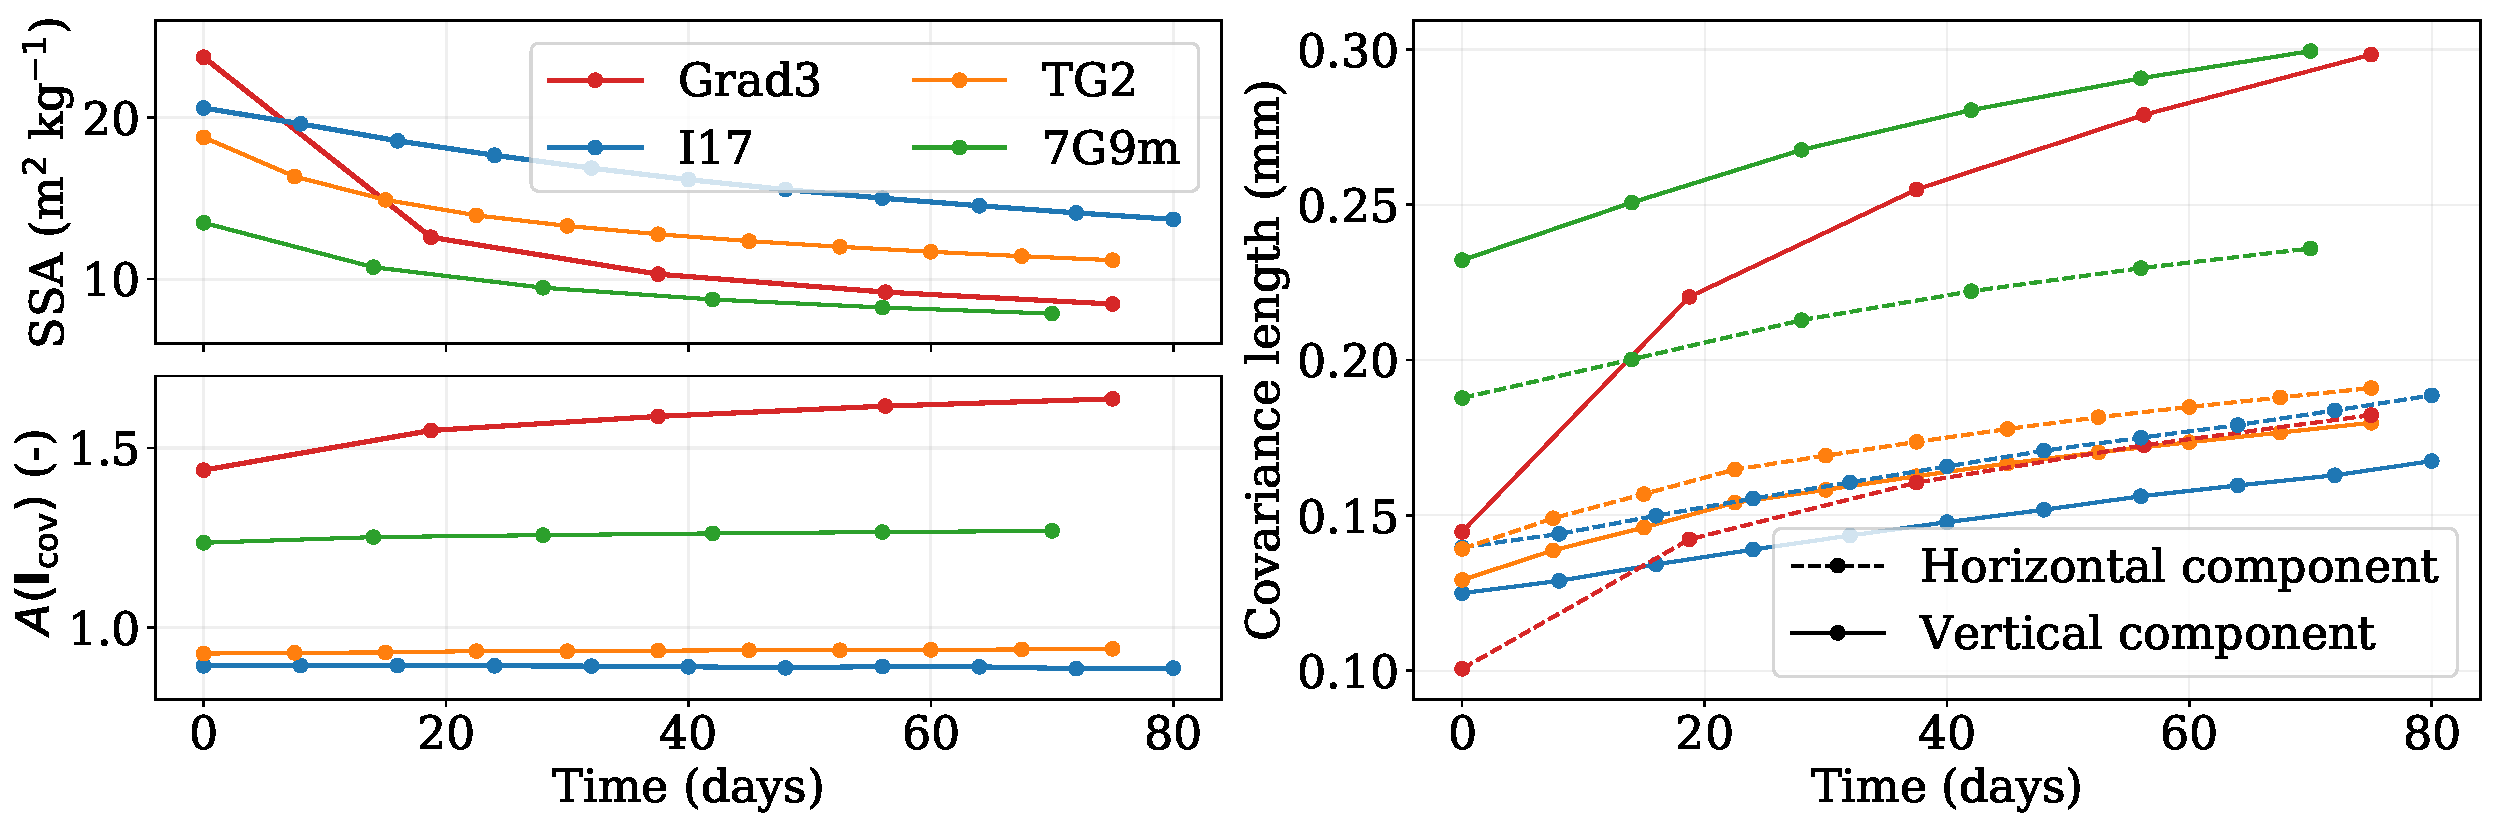
\includegraphics[width=\linewidth]{Figures/4images_microstruct_new.pdf}
    \caption{Time evolution of the microstructural parameters during simulations for the four snow microstructures.}
    \label{fig:4_images_microstruct}
\end{figure}

Figure \ref{fig:4_images_microstruct} shows the evolution of the SSA, covariance lengths, and structural anisotropy of our 4 simulated series. SSA decreases exponentially for each image, as classically reported by ETM experiments and micro-scale models of the literature \cite<see e.g.>{kaempfer_observation_2007, vetter_simulating_2010}. Each series shows different decreasing rates and shapes, ranging from the exponential decrease from 23.7 to 9.2 m$^2$ kg$^{-1}$ for the Grad3 sample to the almost linear slope from 20.6 to 13.7 m$^2$ kg$^{-1}$ for the I17 sample. This difference in decrease rate can be explained by the initial microstructure. Grad3 shows a high initial SSA value, with sharp edges and facets, that leads to a quick and intense evolution (rounding) during the first stage of ETM. In contrast, the sample I17 presents rounded shapes in its initial stage.
The covariance length evolution shows the characteristic increase observed during the ETM, reflecting the growth of snow grains and pores so the overall increase in size of the microstructure \cite{calonne_study_2014, lowe2011interfacial}. Different evolution rates are again observed, from an increase of 0.05 mm for I17 to 0.09 mm for Grad3. Finally, the evolution of the anisotropy ratio provides rather unexpected results. The samples I17 and TG2, presenting a rather isotropic structure with ratio close to 1, show no changes over time. Samples that are initially anisotropic, however, show an increase of their anisotropy with time. The anisotropy of Grad3 increases from 1.44 to 1.62 through the simulation and, in a lesser way, the one of 7G9m evolves from 1.24 to 1.27. By the end of the simulations, the covariance length of Grad3 is about two times larger in the vertical direction than in the horizontal direction. This increase in anisotropy can also be seen in the slices and 3-D images in Figure \ref{fig:evolutions_3D}): the initial vertically elongated ice structure is strengthened as they grow leading to the development of vertical "columns" of ice. 


\subsubsection{Macro-scale transport properties}

\begin{figure}
    \centering
    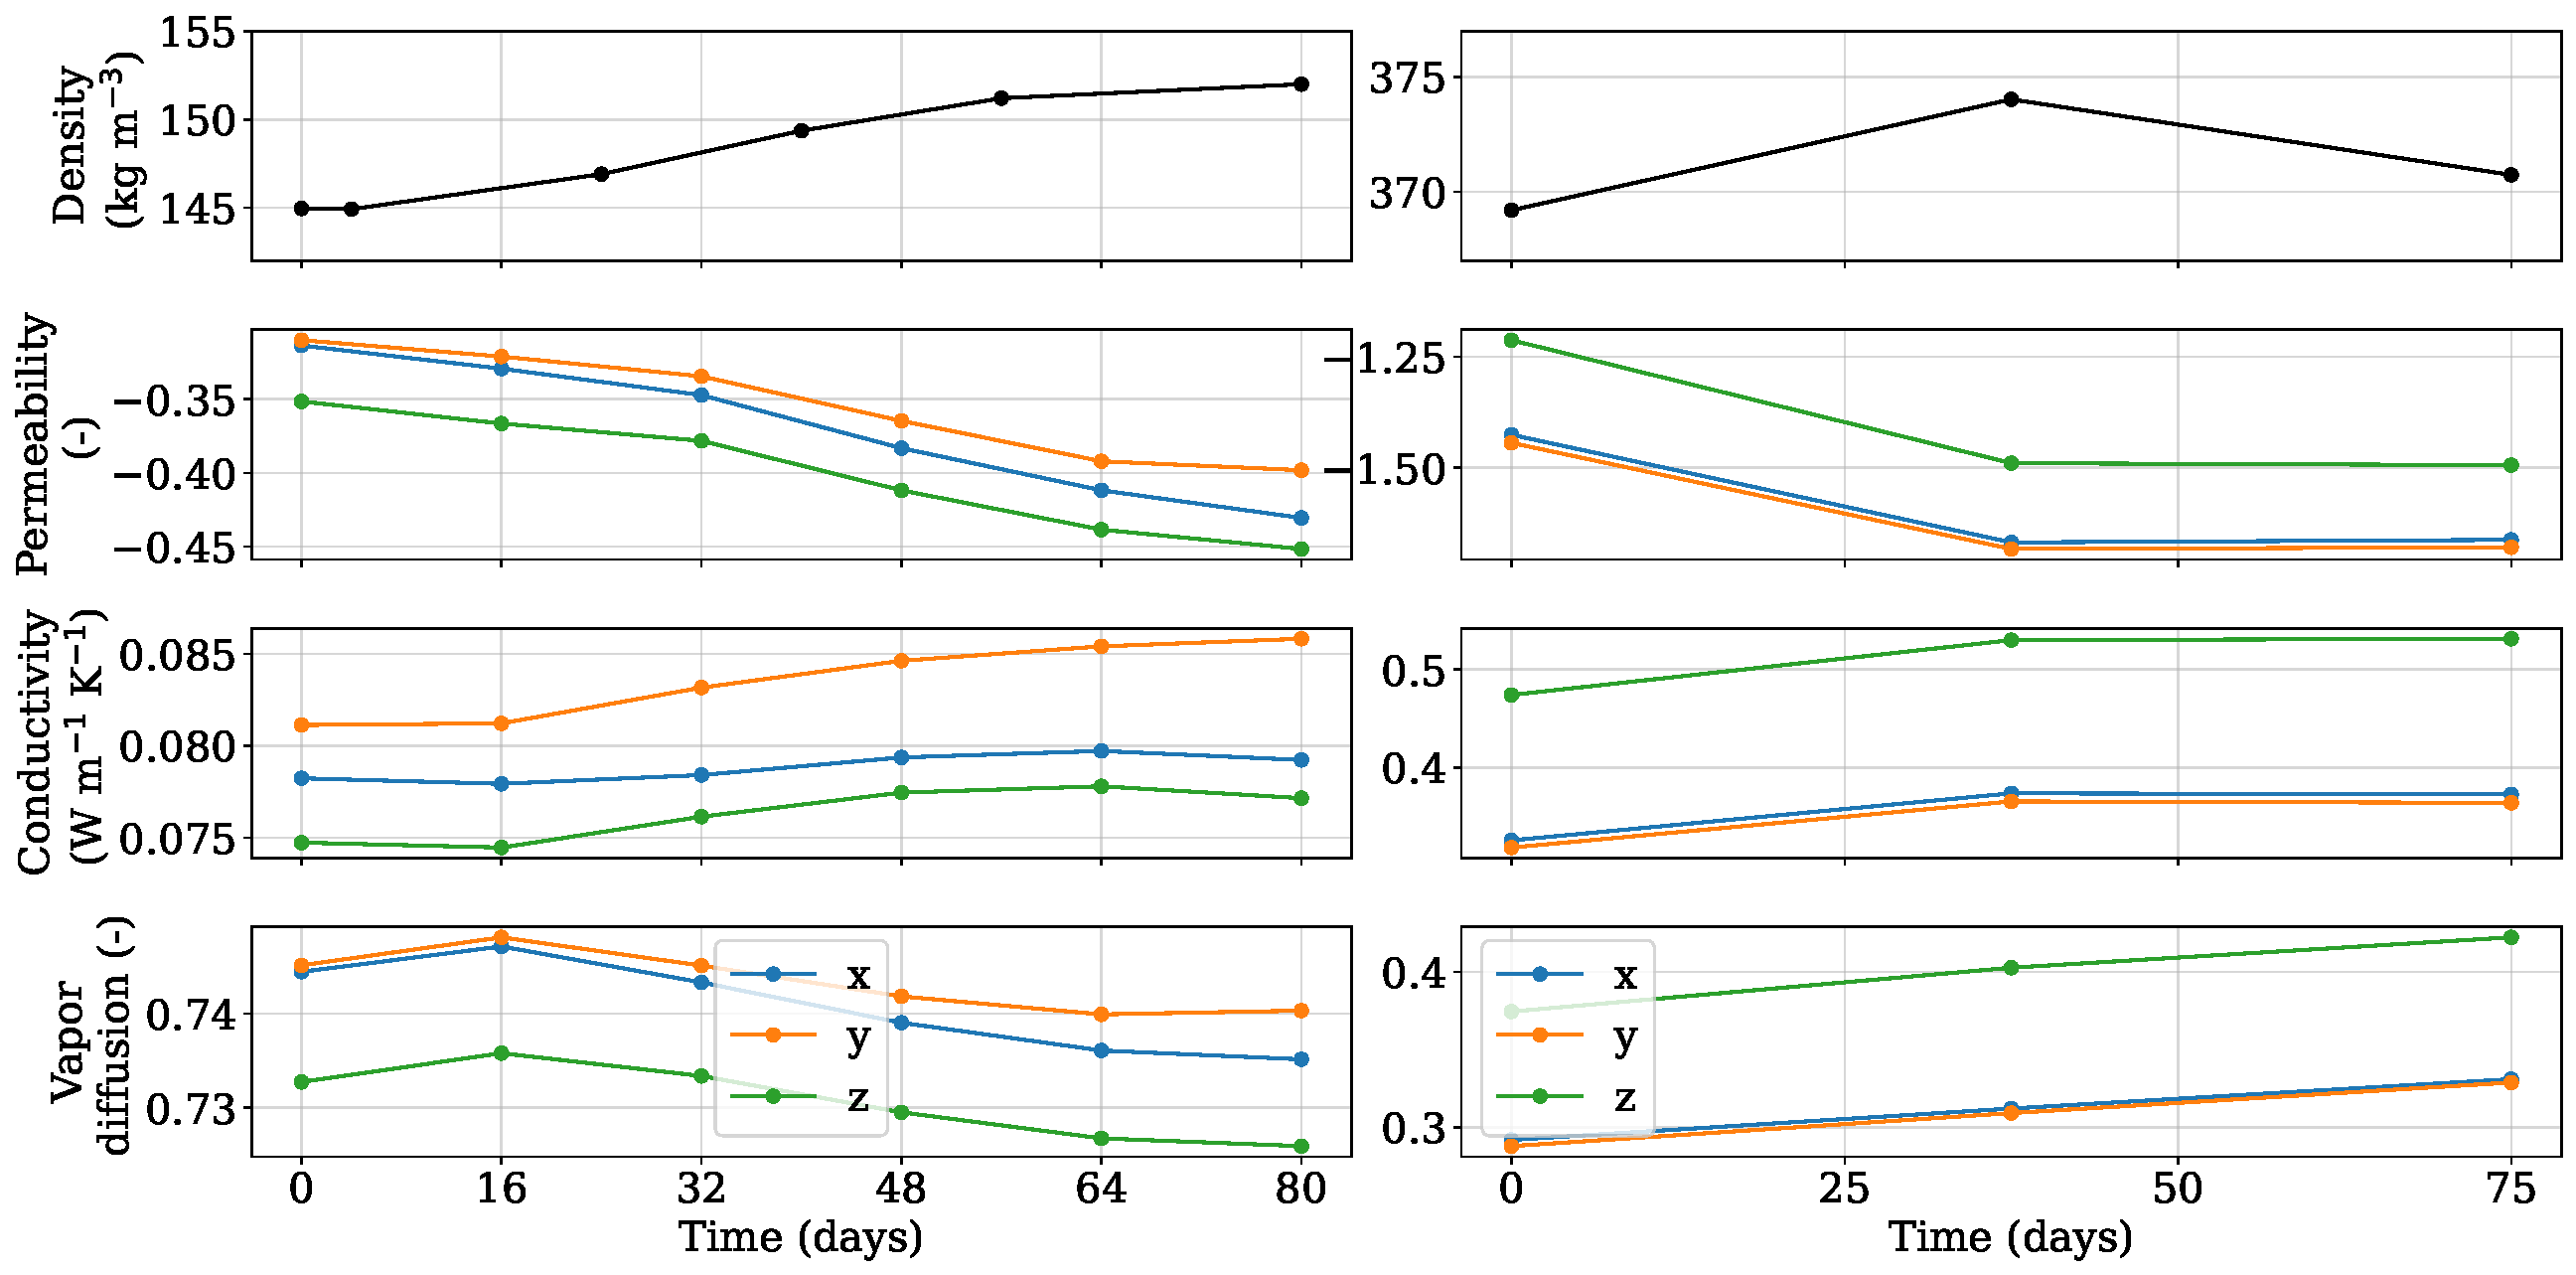
\includegraphics[width=\linewidth]{Figures/4images_transport_temps_court.pdf}
    \caption{Time evolution of density, macroscopic permeability, effective thermal conductivity, and normalized effective coefficient of vapor diffusion for the simulated series fo the I17 sample (left) and Grad3 sample (right). }
    \label{fig:transport_temps}
\end{figure}

In this section we present 3-D estimates of macroscopic transport properties calculated on the simulated series predicting ETM on the 4 microstructures used in the previous section. We focus on the effective thermal conductivity, the effective coefficient of vapor diffusion, and the permeability (Sec. \ref{subsec:methode_physical_appli}).

Figure \ref{fig:transport_temps} presents the evolution of the transport properties for the sample I17 and Grad3. We see that the two samples evolve over different ranges for those properties. The mean normalized permeability decreases over time from -1.36 to -1.61 for Grad3 and from -0.33 to -0.43 for I17. Changes in mean thermal conductivity are small, from 0.37 to 0.42 W m$^{-1}$ K$^{-1}$ for Grad3 and from 0.078 to 0.081 W m$^{-1}$ K$^{-1}$ for I17. Normalized mean vapor diffusion changes are also subtle, with a slight increase for Grad 3, from 0.32 to 0.36, and a slight decrease for I17, from 0.74 to 0.73. Looking at the directional components of the properties, a significant anisotropy is observed for the sample Grad3 (higher vertical components than the horizontal ones) compared to the I17 sample that is rather isotropic.
%
The figure also shows the evolution in density during the simulations. Those density changes are also visible in Figure \ref{fig:Tplot} and show a maximum of 10 kg m$^{-3}$ (3 \%) increase for the TG2 series and a minimum of 4 kg m$^{-3}$ (1 \%) for the Grad3 series. As the model is based on ice mass conservation, these slight density changes correspond to artefacts. They could be caused by discretization effects of the phase-field function, leading to some inaccuracy in the images at the voxel scale (see Sec. \ref{sec:disc} for complementary discussion on this topic).

\begin{figure}
    \centering
    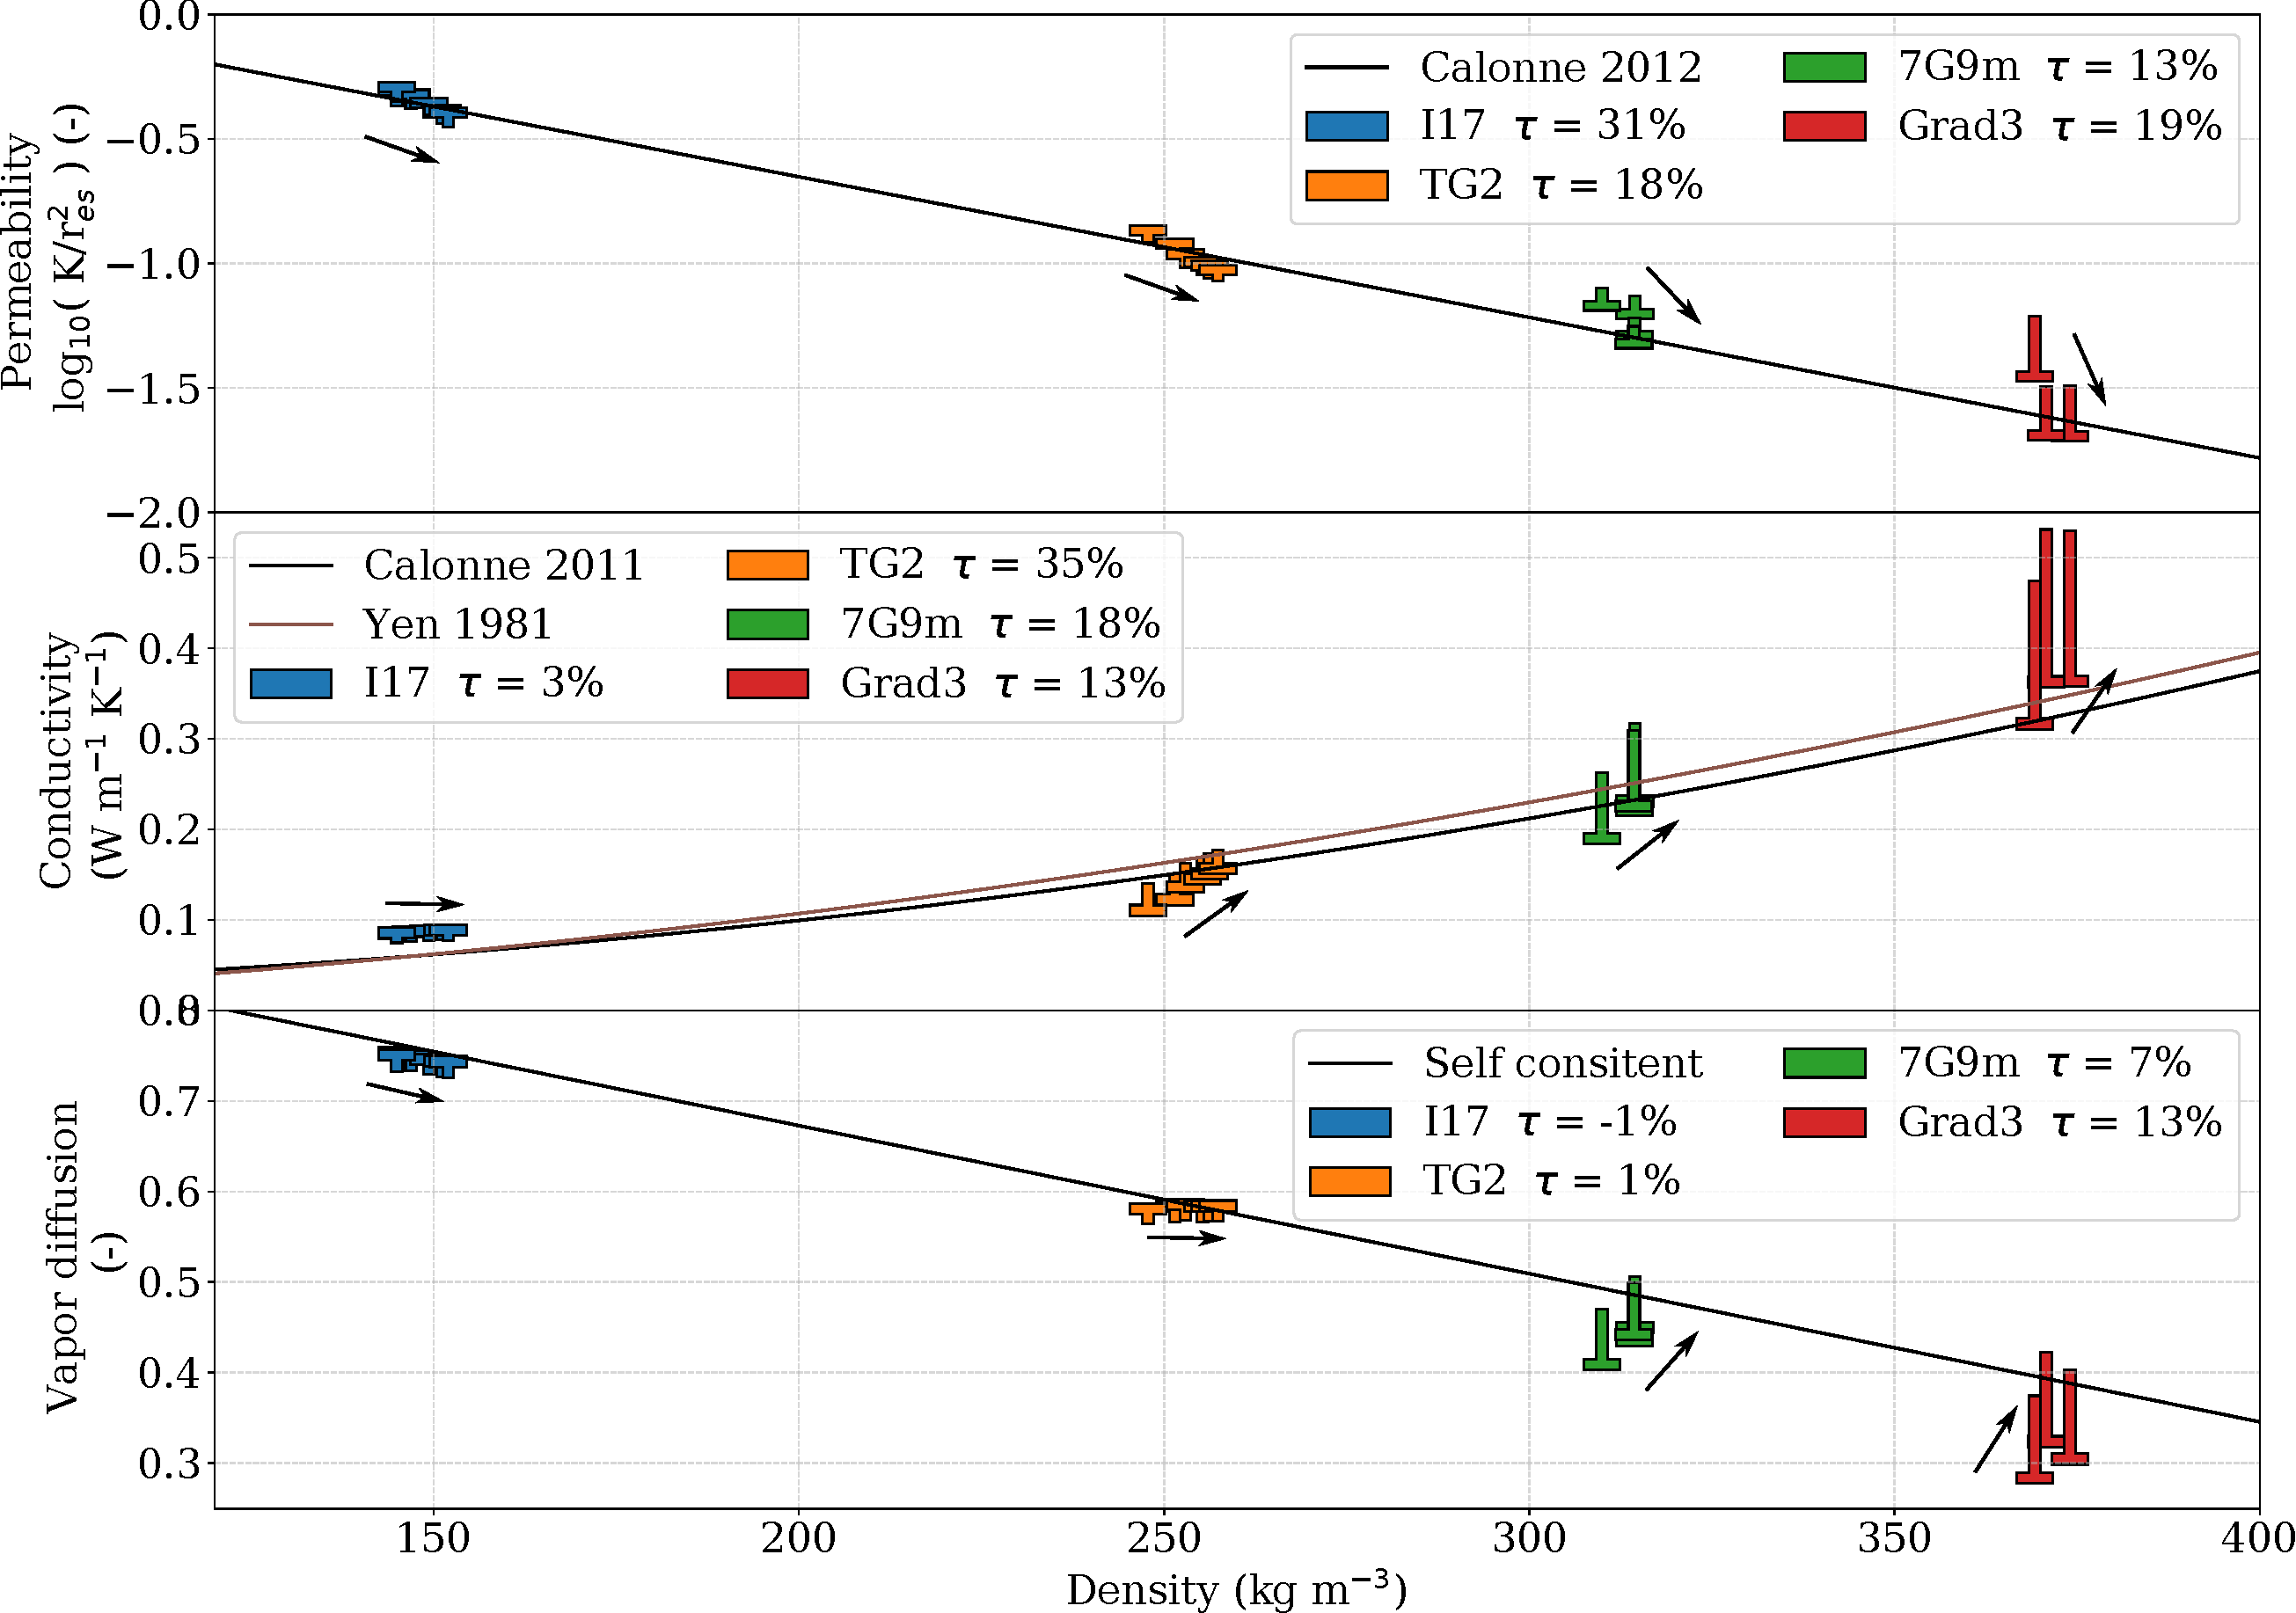
\includegraphics[width=\linewidth]{Figures/tplot_all_arrows.pdf}
    \caption{Effective thermal conductivity, normalized effective vapor diffusion and normalized permeability as a function of density.}
    \label{fig:Tplot}
\end{figure}

Figure \ref{fig:Tplot} shows estimates of the transport properties as a function of density for the four simulated series. Estimates are displayed along with isotropic models based on simplified microstructures (effective coefficient of diffusion \textbf{D}) and current regressions (effective thermal conductivity \textbf{k} and permeability \textbf{K}). The regression from \citeA{calonne_3D_2012} is used for the permeability. For the conductivity we use the regression of \citeA{calonne_numerical_2011} obtained using images of snow spanning a wide range of seasonal snow types. The self-consistent estimate of diffusion for spherical inclusions $D_{\mathrm{SC}}$ from \citeA{calonne_macroscopic_2014} is shown for the coefficient of diffusion: \\
\begin{subequations}
\begin{align}
K_{\mathrm{Calonne\ 2012}}=(3.0 \pm 0.3)\ \exp \left(\left(-0.0130 \pm 0.0003\right) \rho_{\mathrm{s}}\right)
\end{align}
\begin{align}
k_{\mathrm{Calonne\ 2011}}=2.5 \times 10^{-6} \rho_{\mathrm{s}}^{2}-1.23 \times 10^{-4} \rho_{\mathrm{s}}+0.024\end{align}
\begin{align}
D_{\mathrm{SC}} = 1 - \frac{3\rho_s}{2\rho_i}
\end{align}
\end{subequations}
%
 To show the anisotropy of the samples for the displayed properties, the tips and horizontal bars of the ``T" markers represent respectively the vertical and horizontal components. The arrows indicate the evolution direction of the simulated series in time. The relative change between the initial sample and the last step of the simulation $\tau$ is indicated in the legend for each property.

The temporal evolution of the different series in terms of macro-scale properties and density, represented by the arrows and by the relative changes $\tau$, mostly follow the reference parameterizations. This shows that the predicted ETM is in overall good agreement with the expected evolution of those macroscopic properties. 

Grad3 and 7G9m evolution in \textbf{D} are the only series estimates evolving in opposition with the reference parameterization. Those trends can be interpreted as an effect of the microstructure. Indeed, from Figure 9 of \citeA{calonne_macroscopic_2014}, we know that when density increases, $D$ decreases. We also see that for a given density, effective vapor diffusion is smaller for depth hoar samples than for faceted crystals and even more for rounded grains samples. As Grad3 and 7G9m samples evolve from depth hoar to more rounded shapes (Figure \ref{fig:evolutions_3D}) while increasing in density, the changes in microstructure and in density have an opposite effect on the coefficient of diffusion, and the microstructure influence could overcome the increase in density. \\
This microstructure influence is also present for the permeability, as seen in Figure 1 of \citeA{calonne_3D_2012}. In this figure, the permeability regression decreases when the density increases, but at a given density, depth hoar seems to have higher permeability than faceted crystals or rounded grains. For Grad3 and 7G9m, both the microstructure and the density evolution lead to a decreasing permeability.\\
For the thermal conductivity, the microstructure impact is not that distinct in the Figure 1 of \citeA{calonne_numerical_2011} and the simulations seem to follow the regression in Figure \ref{fig:Tplot}.


\section{Discussion}
\label{sec:disc}

This work provides a new ETM model applicable on real 3-D tomographic images. This optimized model has been calibrated and evaluated using experimental ETM series, and used for metamorphism prediction on a set of different microstructures by characterizing the images using numerous microstructural and macro-scale transport properties.

Having the results in mind, it is worth while discussing the model artefacts in some more details. 
% density increase ------------

\begin{figure}
    \centering
    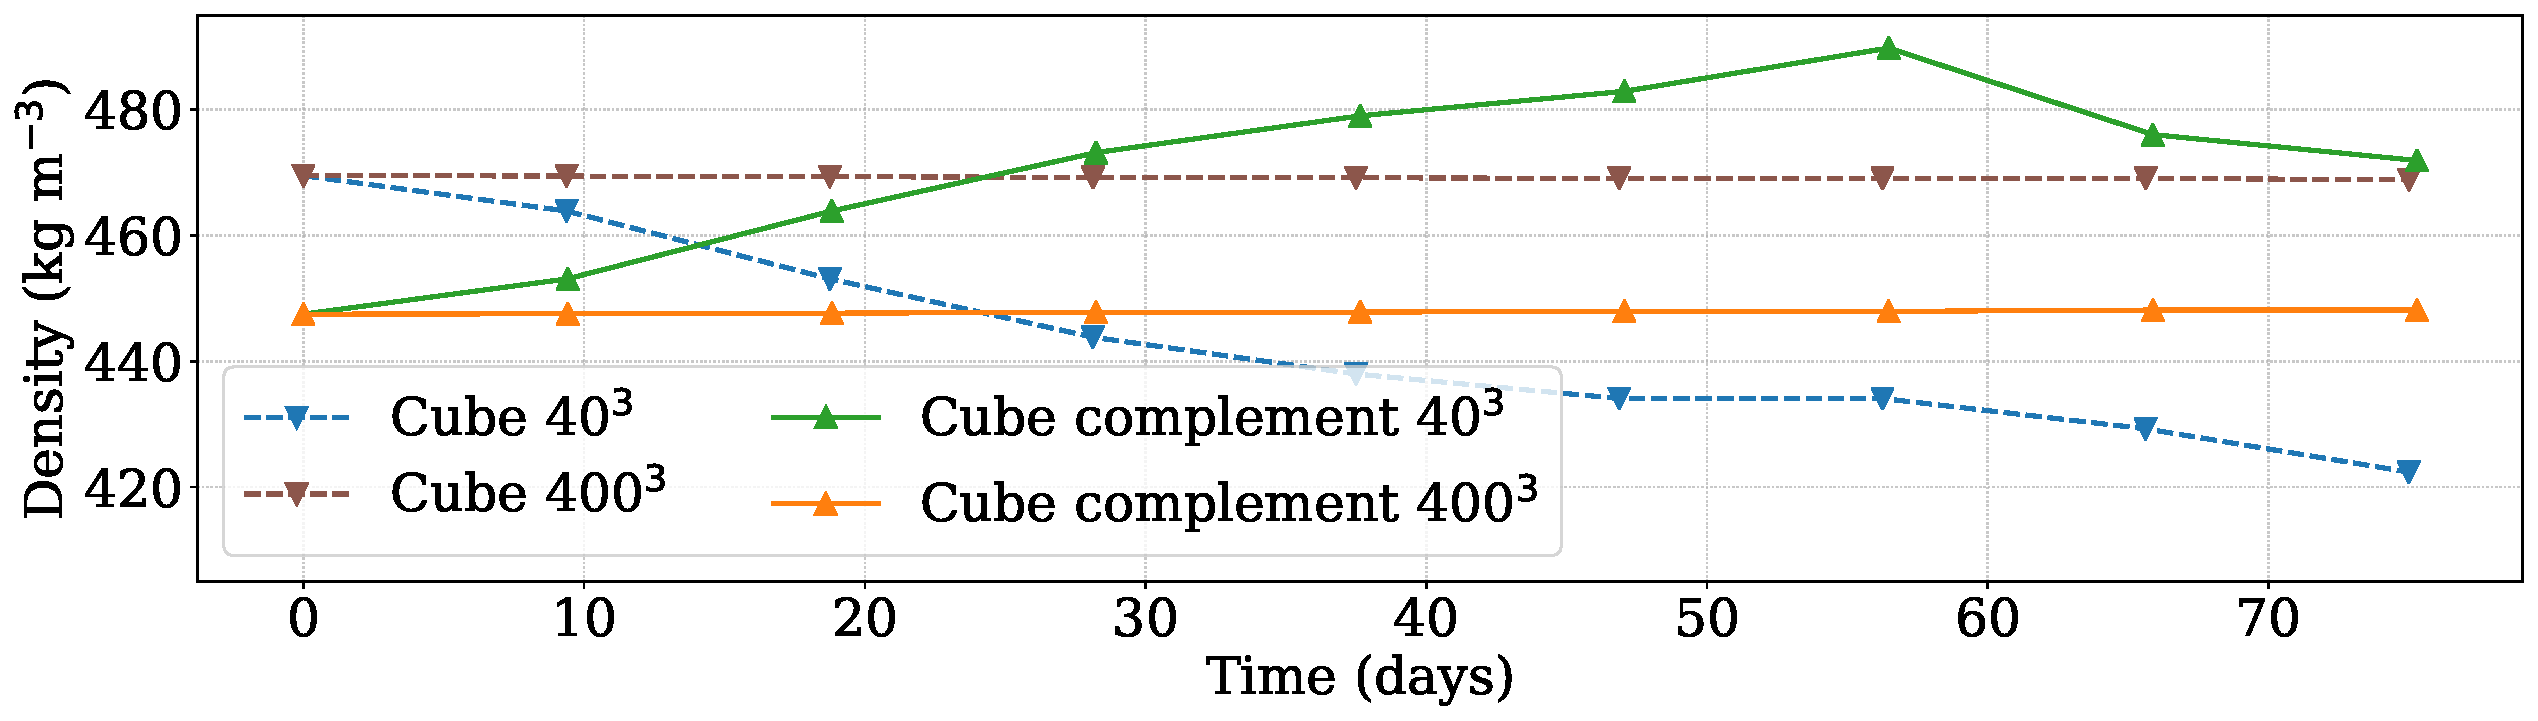
\includegraphics[width=0.9\linewidth]{Figures/cubes_compl_density_propre.pdf}
    \caption{Influence of the image resolution on the modeled density evolution: example of a cube surrounded by air and its complementary image.}
    \label{fig:cubes}
\end{figure}

For our 4 simulated series, we observe an increase in density in Figure \ref{fig:Tplot} and Figure \ref{fig:transport_temps} whereas the model does not simulate changes in density. This is thus an artefact that contradicts mass conservation. This error seems to occur during the binarization of the phase-field function. At the end of the simulation, the continuous interface of the phase-field function is approximated by air and ice voxels of finite length. This step can induce at most an error of one layer of voxels on the ice-air interface. Those voxels constitute 9 \% of TG2 and 6 \% of Grad3 ice phase, which cover the mass gain observed in the simulations. In Figure \ref{fig:cubes}, we run the model on four different images: a cube surrounded by air with a size of 40$^3$ voxels; the same cube with a size of 400$^3$ voxels; the complement of the cube - a cube of air surrounded by ice - with a size of 40$^3$ voxels and the same image at 400$^3$ voxels. The idea is to test the simulated density evolution for different resolutions and shapes, with an image presenting convex shapes (the cube) and with one presenting concave shapes (the cube complement). We see clearly in the graph that for a fine resolution, the density is stable in time, whereas for a coarser resolution, the density has an erratic progression, with gain of about 10 \%. Indeed, the finer the resolution, the thinner the layer of voxel of the ice surface and the lower the error. In terms of ratio between the object length (covariance length) and the voxel size, the data of Figure \ref{fig:Tplot} are similar to the cube and the cube complement of 40$^3$ voxels. %Furthermore, the ratio between the elements size and the resolution gets larger from I17, to TG2 to Grad3 and to 7G9m, as the density changes gets smaller.
In our data, the maximum density increase is of 3 \% for the TG2 series. It is however within the precision range of snow density measurements such as the box cutter that have a precision of 5 \% \cite{proksch2016intercomparison}. Moreover, the settling process has an important role in ETM. For example in \citeA{flin_three-dimensional_2004} the density increases of 60 \% in 80 days. Thus, the artefact is small in comparison with the measurement precision and the observed settling, and it enables to investigate the impact of slight density variations.\\

% ---------------------------- 1ere itération
%In Figure \ref{fig:Tplot} we also see a gap between the first image of each series, which is the experimental one, and the simulated ones. This gap can be caused by the first step of the algorithm, which modify the image to conform it to the model constraints.\\
% Calibration et validation -------------
Other points worth discussing are the calibration and the model evaluation. The condensation coefficient $\alpha$ is approximated by an isotropic constant value. This hypothesis has however never been verified and $\alpha$ seems to have numerous dependencies. For example, \citeA{libbrecht2019snow} highlighted dependencies in temperature, supersaturation and crystalline orientation. The author measured basal and prismatic $\alpha$ on growing snow crystal, with results between $10^{-3}$ and $10^{-1}$.
In our calibration process, the $\alpha$ parameter is determined using an experimental series of \citeA{flin_three-dimensional_2004} obtained at -2$^\circ$C. In view of $\alpha$ complex dependencies, its calibrated value can incorporate non-modeled experimental conditions (temperature variations, vapor diffusion...).
To test and evaluate the calibration, we use the equi-temperature time series of \citeA{hagenmuller_motion_2019}, also realized at -2$^\circ$C. As the experimental time series is very short compared to \citeA{flin_three-dimensional_2004} (3 days versus 28 days), the comparison with the microstructural properties is relatively weak and would benefit of a comparison with a longer independent series of ETM. 
% ------------ Prediction

Finally, concerning the ETM prediction, the notable result is the enhancement of structural anisotropy for the very anisotropic depth hoar sample Grad3. The Grad3 experimental sample (DH) has a particular morphology: it presents a dense structure with many intricate angular shapes. On a larger scale, the sample seems to be organized into vertical shapes. With ETM, the general smoothing seems to remove small shapes to let the general structure appear with the formation of wide vertical columns, increasing the value of the structural anisotropy. A conservation of the anisotropy is also observed for 7G9m, without significant increase. The enhancement of structural anisotropy in the Grad3 sample is a rather unexpected result as such feature was never reported in previous studies and one could think that a sample presenting a strong anisotropy would tend to lose it for the benefit of a more isotropic structure as classically observed in equi-temperature conditions. One can still question if this result is particular to this only two-scale sample or if it can be generalized for any strongly anisotropic sample. 

\section{Conclusion}
\label{sec:conclusion}

A snow ETM model, based on the work of \citeA{bretin_phase-field_2019} was applied to snow images obtained by X-ray tomography to study the impact on the microstructural and transport properties. The model was calibrated to experimental data at – 2°C by fitting the SSA of the series from \citeA{flin_three-dimensional_2004} to the simulation. A value of the condensation coefficient $\alpha$ was derived: $\alpha = ( 9.8 \pm 0.7) 10^{-4}$. The calibrated model was then evaluated with the independent experimental series of \citeA{hagenmuller_motion_2019} by looking at microstructural properties such as the SSA, the covariance length, the structural anisotropy and the mean curvature. As this evaluation raised very encouraging results, the model Snow-3D was used to model ETM on four different snow microstructures from experimental samples. The four simulated time series were used to analyze microstructural parameters (SSA, covariance length, structural anisotropy) and physical effective transport properties (thermal conductivity, vapor diffusivity and permeability). Those results are in good agreement with current models and regressions. They also exhibit the influence of the microstructure on micro-scale (structural anisotropy) and macro-scale (effective coefficient of diffusion) phenomenon. For example, we observed an enhancement of the structural anisotropy in the case of initially anisotropic microstructures. It questions the idea that isotropic conditions tend to remove the snow structure anisotropy. This model is a step forward for modeling ETM at the pore scale. Future studies will focus on implementing the settling process and water vapor transport in pores, as well on studying the condensation coefficient depending on various parameters such as the temperature.

\acknowledgments
The 3SR lab is part of the Labex Tec 21 (investissements d'Avenir, Grand Agreement ANR-11-LABX-0030). CNRM/CEN is part of Labex OSUG@2020 (Investissements d'Avenir, Grand ANR-10-LABX-0056). This research has been supported by the MiMESis-3D ANR project (ANR-19-CE01-0009).

\bibliography{Snow3D}




\end{document}


